\documentclass[11pt]{article}

% Shared notes settings for Applied Machine Learning lectures (UPES).
% Keep this file free of \documentclass to allow reuse via \input.

\usepackage[utf8]{inputenc}
\usepackage[T1]{fontenc}
\usepackage{lmodern}          % scalable T1 fonts; without this pdflatex falls back
\input{glyphtounicode}        % to bitmapped EC Type 3 and the PDFs are neither
\pdfgentounicode=1            % searchable nor screen-reader friendly
\usepackage[a4paper,margin=1in]{geometry}
\usepackage{hyperref}
\usepackage{xurl}
\usepackage{booktabs}
\usepackage{amsmath}
\usepackage{amssymb}
\usepackage{listings}
\usepackage{xcolor}
\usepackage{enumitem}
\usepackage{parskip}

% Code listings (Python-oriented for this subject).
\lstset{
  language=Python,
  basicstyle=\ttfamily\small,
  keywordstyle=\color{blue},
  commentstyle=\color{gray},
  stringstyle=\color{teal},
  showstringspaces=false,
  columns=fullflexible,
  frame=single,
  framerule=0.2pt,
  breaklines=true
}

\setlist[itemize]{topsep=0.3em,itemsep=0.2em}
\setlist[enumerate]{topsep=0.3em,itemsep=0.2em}

% Simple per-section source line.
\newcommand{\notesources}[1]{\par\noindent{\small\color{gray}\textit{Sources:} \sloppy #1\par}}

% Unit-wise source strings for this subject (used by slides + notes).
% Path is relative to the lecture `latex/` folder (the compilation CWD).
\IfFileExists{../../../_shared/aml-sources.tex}{%
  % Source strings for Applied Machine Learning (CSAI2017P) — used by slides + notes.
% Prescribed texts and reference books are taken from the course syllabus.
% Support texts are the author-hosted open-access editions:
%   statlearning.com            (ISL with Python)
%   probml.github.io/pml-book   (Murphy, Probabilistic Machine Learning)
%   d2l.ai                      (Dive into Deep Learning)
%   mml-book.github.io          (Mathematics for Machine Learning)

\newcommand{\AMLRepoURL}{https://github.com/tali7c/Applied-Machine-Learning}

% --- prescribed -------------------------------------------------------------
\newcommand{\AMLPrescribed}{%
M\"uller and Guido, \textit{Introduction to Machine Learning with Python}, O'Reilly, 2016.;%
Bishop, \textit{Pattern Recognition and Machine Learning}, Springer, 2006.;%
Murphy, \textit{Machine Learning: A Probabilistic Perspective}, MIT Press, 2012.;%
Han, Kamber and Pei, \textit{Data Mining: Concepts and Techniques} (3e), Morgan Kaufmann, 2012.%
}

% --- unit-wise ---------------------------------------------------------------
\newcommand{\AMLUnitISources}{%
M\"uller and Guido, \textit{Introduction to Machine Learning with Python}, Ch. 1.;%
Bishop, \textit{Pattern Recognition and Machine Learning}, Ch. 1.;%
Murphy, \textit{Probabilistic Machine Learning: An Introduction}, MIT Press, 2022, Ch. 1.;%
Mitchell, \textit{Machine Learning}, McGraw Hill, 1997, Ch. 1.;%
Scikit-learn documentation, accessed 2026-08-04.%
}

\newcommand{\AMLUnitIISources}{%
Bishop, \textit{Pattern Recognition and Machine Learning}, \S1.5, \S4.3, \S7.1.;%
Zhang, Lipton, Li and Smola, \textit{Dive into Deep Learning}, \S3.4.;%
Shalev-Shwartz and Ben-David, \textit{Understanding Machine Learning}, Ch. 15.;%
Murphy, \textit{Probabilistic Machine Learning: An Introduction}, Ch. 5.%
}

\newcommand{\AMLUnitIIISources}{%
Zhang, Lipton, Li and Smola, \textit{Dive into Deep Learning}, Ch. 12 (Optimization Algorithms).;%
Deisenroth, Faisal and Ong, \textit{Mathematics for Machine Learning}, Ch. 7.;%
Kingma and Ba, ``Adam: A Method for Stochastic Optimization,'' ICLR 2015.;%
Ruder, ``An overview of gradient descent optimization algorithms,'' arXiv:1609.04747, 2016.%
}

\newcommand{\AMLUnitIVSources}{%
Han, Kamber and Pei, \textit{Data Mining: Concepts and Techniques} (3e), Ch. 3.;%
M\"uller and Guido, \textit{Introduction to Machine Learning with Python}, Ch. 3--4.;%
James, Witten, Hastie, Tibshirani and Taylor, \textit{An Introduction to Statistical Learning with Python}, Ch. 5--6, 12.;%
Scikit-learn documentation (preprocessing, model selection), accessed 2026-08-04.%
}

\newcommand{\AMLUnitVSources}{%
James et al., \textit{An Introduction to Statistical Learning with Python}, Ch. 3--6.;%
Bishop, \textit{Pattern Recognition and Machine Learning}, Ch. 3.;%
Deisenroth, Faisal and Ong, \textit{Mathematics for Machine Learning}, Ch. 9.;%
M\"uller and Guido, \textit{Introduction to Machine Learning with Python}, \S2.3.%
}

\newcommand{\AMLUnitVISources}{%
Han, Kamber and Pei, \textit{Data Mining: Concepts and Techniques} (3e), Ch. 8--9.;%
James et al., \textit{An Introduction to Statistical Learning with Python}, Ch. 8--9.;%
Bishop, \textit{Pattern Recognition and Machine Learning}, Ch. 4--5, 7, 14.;%
Zhang et al., \textit{Dive into Deep Learning}, Ch. 5.%
}

\newcommand{\AMLUnitVIISources}{%
Han, Kamber and Pei, \textit{Data Mining: Concepts and Techniques} (3e), Ch. 10.;%
James et al., \textit{An Introduction to Statistical Learning with Python}, Ch. 12.;%
M\"uller and Guido, \textit{Introduction to Machine Learning with Python}, \S3.5.;%
Ester, Kriegel, Sander and Xu, ``A density-based algorithm for discovering clusters (DBSCAN),'' KDD 1996.%
}

\newcommand{\AMLLabSources}{%
M\"uller and Guido, \textit{Introduction to Machine Learning with Python}, companion notebooks.;%
McKinney, \textit{Python for Data Analysis} (3e), O'Reilly, 2022.;%
Scikit-learn user guide, accessed 2026-08-04.;%
Matplotlib and Seaborn documentation, accessed 2026-08-04.%
}
%
}{%
  % Faculty copies live under `private/` so their compile CWD is different.
  \IfFileExists{../../../../public/_shared/aml-sources.tex}{%
    % Source strings for Applied Machine Learning (CSAI2017P) — used by slides + notes.
% Prescribed texts and reference books are taken from the course syllabus.
% Support texts are the author-hosted open-access editions:
%   statlearning.com            (ISL with Python)
%   probml.github.io/pml-book   (Murphy, Probabilistic Machine Learning)
%   d2l.ai                      (Dive into Deep Learning)
%   mml-book.github.io          (Mathematics for Machine Learning)

\newcommand{\AMLRepoURL}{https://github.com/tali7c/Applied-Machine-Learning}

% --- prescribed -------------------------------------------------------------
\newcommand{\AMLPrescribed}{%
M\"uller and Guido, \textit{Introduction to Machine Learning with Python}, O'Reilly, 2016.;%
Bishop, \textit{Pattern Recognition and Machine Learning}, Springer, 2006.;%
Murphy, \textit{Machine Learning: A Probabilistic Perspective}, MIT Press, 2012.;%
Han, Kamber and Pei, \textit{Data Mining: Concepts and Techniques} (3e), Morgan Kaufmann, 2012.%
}

% --- unit-wise ---------------------------------------------------------------
\newcommand{\AMLUnitISources}{%
M\"uller and Guido, \textit{Introduction to Machine Learning with Python}, Ch. 1.;%
Bishop, \textit{Pattern Recognition and Machine Learning}, Ch. 1.;%
Murphy, \textit{Probabilistic Machine Learning: An Introduction}, MIT Press, 2022, Ch. 1.;%
Mitchell, \textit{Machine Learning}, McGraw Hill, 1997, Ch. 1.;%
Scikit-learn documentation, accessed 2026-08-04.%
}

\newcommand{\AMLUnitIISources}{%
Bishop, \textit{Pattern Recognition and Machine Learning}, \S1.5, \S4.3, \S7.1.;%
Zhang, Lipton, Li and Smola, \textit{Dive into Deep Learning}, \S3.4.;%
Shalev-Shwartz and Ben-David, \textit{Understanding Machine Learning}, Ch. 15.;%
Murphy, \textit{Probabilistic Machine Learning: An Introduction}, Ch. 5.%
}

\newcommand{\AMLUnitIIISources}{%
Zhang, Lipton, Li and Smola, \textit{Dive into Deep Learning}, Ch. 12 (Optimization Algorithms).;%
Deisenroth, Faisal and Ong, \textit{Mathematics for Machine Learning}, Ch. 7.;%
Kingma and Ba, ``Adam: A Method for Stochastic Optimization,'' ICLR 2015.;%
Ruder, ``An overview of gradient descent optimization algorithms,'' arXiv:1609.04747, 2016.%
}

\newcommand{\AMLUnitIVSources}{%
Han, Kamber and Pei, \textit{Data Mining: Concepts and Techniques} (3e), Ch. 3.;%
M\"uller and Guido, \textit{Introduction to Machine Learning with Python}, Ch. 3--4.;%
James, Witten, Hastie, Tibshirani and Taylor, \textit{An Introduction to Statistical Learning with Python}, Ch. 5--6, 12.;%
Scikit-learn documentation (preprocessing, model selection), accessed 2026-08-04.%
}

\newcommand{\AMLUnitVSources}{%
James et al., \textit{An Introduction to Statistical Learning with Python}, Ch. 3--6.;%
Bishop, \textit{Pattern Recognition and Machine Learning}, Ch. 3.;%
Deisenroth, Faisal and Ong, \textit{Mathematics for Machine Learning}, Ch. 9.;%
M\"uller and Guido, \textit{Introduction to Machine Learning with Python}, \S2.3.%
}

\newcommand{\AMLUnitVISources}{%
Han, Kamber and Pei, \textit{Data Mining: Concepts and Techniques} (3e), Ch. 8--9.;%
James et al., \textit{An Introduction to Statistical Learning with Python}, Ch. 8--9.;%
Bishop, \textit{Pattern Recognition and Machine Learning}, Ch. 4--5, 7, 14.;%
Zhang et al., \textit{Dive into Deep Learning}, Ch. 5.%
}

\newcommand{\AMLUnitVIISources}{%
Han, Kamber and Pei, \textit{Data Mining: Concepts and Techniques} (3e), Ch. 10.;%
James et al., \textit{An Introduction to Statistical Learning with Python}, Ch. 12.;%
M\"uller and Guido, \textit{Introduction to Machine Learning with Python}, \S3.5.;%
Ester, Kriegel, Sander and Xu, ``A density-based algorithm for discovering clusters (DBSCAN),'' KDD 1996.%
}

\newcommand{\AMLLabSources}{%
M\"uller and Guido, \textit{Introduction to Machine Learning with Python}, companion notebooks.;%
McKinney, \textit{Python for Data Analysis} (3e), O'Reilly, 2022.;%
Scikit-learn user guide, accessed 2026-08-04.;%
Matplotlib and Seaborn documentation, accessed 2026-08-04.%
}
%
  }{%
    % Question papers live at `private/<family>/<instrument>/`.
    \IfFileExists{../../../public/_shared/aml-sources.tex}{%
      % Source strings for Applied Machine Learning (CSAI2017P) — used by slides + notes.
% Prescribed texts and reference books are taken from the course syllabus.
% Support texts are the author-hosted open-access editions:
%   statlearning.com            (ISL with Python)
%   probml.github.io/pml-book   (Murphy, Probabilistic Machine Learning)
%   d2l.ai                      (Dive into Deep Learning)
%   mml-book.github.io          (Mathematics for Machine Learning)

\newcommand{\AMLRepoURL}{https://github.com/tali7c/Applied-Machine-Learning}

% --- prescribed -------------------------------------------------------------
\newcommand{\AMLPrescribed}{%
M\"uller and Guido, \textit{Introduction to Machine Learning with Python}, O'Reilly, 2016.;%
Bishop, \textit{Pattern Recognition and Machine Learning}, Springer, 2006.;%
Murphy, \textit{Machine Learning: A Probabilistic Perspective}, MIT Press, 2012.;%
Han, Kamber and Pei, \textit{Data Mining: Concepts and Techniques} (3e), Morgan Kaufmann, 2012.%
}

% --- unit-wise ---------------------------------------------------------------
\newcommand{\AMLUnitISources}{%
M\"uller and Guido, \textit{Introduction to Machine Learning with Python}, Ch. 1.;%
Bishop, \textit{Pattern Recognition and Machine Learning}, Ch. 1.;%
Murphy, \textit{Probabilistic Machine Learning: An Introduction}, MIT Press, 2022, Ch. 1.;%
Mitchell, \textit{Machine Learning}, McGraw Hill, 1997, Ch. 1.;%
Scikit-learn documentation, accessed 2026-08-04.%
}

\newcommand{\AMLUnitIISources}{%
Bishop, \textit{Pattern Recognition and Machine Learning}, \S1.5, \S4.3, \S7.1.;%
Zhang, Lipton, Li and Smola, \textit{Dive into Deep Learning}, \S3.4.;%
Shalev-Shwartz and Ben-David, \textit{Understanding Machine Learning}, Ch. 15.;%
Murphy, \textit{Probabilistic Machine Learning: An Introduction}, Ch. 5.%
}

\newcommand{\AMLUnitIIISources}{%
Zhang, Lipton, Li and Smola, \textit{Dive into Deep Learning}, Ch. 12 (Optimization Algorithms).;%
Deisenroth, Faisal and Ong, \textit{Mathematics for Machine Learning}, Ch. 7.;%
Kingma and Ba, ``Adam: A Method for Stochastic Optimization,'' ICLR 2015.;%
Ruder, ``An overview of gradient descent optimization algorithms,'' arXiv:1609.04747, 2016.%
}

\newcommand{\AMLUnitIVSources}{%
Han, Kamber and Pei, \textit{Data Mining: Concepts and Techniques} (3e), Ch. 3.;%
M\"uller and Guido, \textit{Introduction to Machine Learning with Python}, Ch. 3--4.;%
James, Witten, Hastie, Tibshirani and Taylor, \textit{An Introduction to Statistical Learning with Python}, Ch. 5--6, 12.;%
Scikit-learn documentation (preprocessing, model selection), accessed 2026-08-04.%
}

\newcommand{\AMLUnitVSources}{%
James et al., \textit{An Introduction to Statistical Learning with Python}, Ch. 3--6.;%
Bishop, \textit{Pattern Recognition and Machine Learning}, Ch. 3.;%
Deisenroth, Faisal and Ong, \textit{Mathematics for Machine Learning}, Ch. 9.;%
M\"uller and Guido, \textit{Introduction to Machine Learning with Python}, \S2.3.%
}

\newcommand{\AMLUnitVISources}{%
Han, Kamber and Pei, \textit{Data Mining: Concepts and Techniques} (3e), Ch. 8--9.;%
James et al., \textit{An Introduction to Statistical Learning with Python}, Ch. 8--9.;%
Bishop, \textit{Pattern Recognition and Machine Learning}, Ch. 4--5, 7, 14.;%
Zhang et al., \textit{Dive into Deep Learning}, Ch. 5.%
}

\newcommand{\AMLUnitVIISources}{%
Han, Kamber and Pei, \textit{Data Mining: Concepts and Techniques} (3e), Ch. 10.;%
James et al., \textit{An Introduction to Statistical Learning with Python}, Ch. 12.;%
M\"uller and Guido, \textit{Introduction to Machine Learning with Python}, \S3.5.;%
Ester, Kriegel, Sander and Xu, ``A density-based algorithm for discovering clusters (DBSCAN),'' KDD 1996.%
}

\newcommand{\AMLLabSources}{%
M\"uller and Guido, \textit{Introduction to Machine Learning with Python}, companion notebooks.;%
McKinney, \textit{Python for Data Analysis} (3e), O'Reilly, 2022.;%
Scikit-learn user guide, accessed 2026-08-04.;%
Matplotlib and Seaborn documentation, accessed 2026-08-04.%
}
%
    }{%
      % Marking schemes live at `private/solutions/<family>/<id>/latex/`.
      \IfFileExists{../../../../../public/_shared/aml-sources.tex}{%
        % Source strings for Applied Machine Learning (CSAI2017P) — used by slides + notes.
% Prescribed texts and reference books are taken from the course syllabus.
% Support texts are the author-hosted open-access editions:
%   statlearning.com            (ISL with Python)
%   probml.github.io/pml-book   (Murphy, Probabilistic Machine Learning)
%   d2l.ai                      (Dive into Deep Learning)
%   mml-book.github.io          (Mathematics for Machine Learning)

\newcommand{\AMLRepoURL}{https://github.com/tali7c/Applied-Machine-Learning}

% --- prescribed -------------------------------------------------------------
\newcommand{\AMLPrescribed}{%
M\"uller and Guido, \textit{Introduction to Machine Learning with Python}, O'Reilly, 2016.;%
Bishop, \textit{Pattern Recognition and Machine Learning}, Springer, 2006.;%
Murphy, \textit{Machine Learning: A Probabilistic Perspective}, MIT Press, 2012.;%
Han, Kamber and Pei, \textit{Data Mining: Concepts and Techniques} (3e), Morgan Kaufmann, 2012.%
}

% --- unit-wise ---------------------------------------------------------------
\newcommand{\AMLUnitISources}{%
M\"uller and Guido, \textit{Introduction to Machine Learning with Python}, Ch. 1.;%
Bishop, \textit{Pattern Recognition and Machine Learning}, Ch. 1.;%
Murphy, \textit{Probabilistic Machine Learning: An Introduction}, MIT Press, 2022, Ch. 1.;%
Mitchell, \textit{Machine Learning}, McGraw Hill, 1997, Ch. 1.;%
Scikit-learn documentation, accessed 2026-08-04.%
}

\newcommand{\AMLUnitIISources}{%
Bishop, \textit{Pattern Recognition and Machine Learning}, \S1.5, \S4.3, \S7.1.;%
Zhang, Lipton, Li and Smola, \textit{Dive into Deep Learning}, \S3.4.;%
Shalev-Shwartz and Ben-David, \textit{Understanding Machine Learning}, Ch. 15.;%
Murphy, \textit{Probabilistic Machine Learning: An Introduction}, Ch. 5.%
}

\newcommand{\AMLUnitIIISources}{%
Zhang, Lipton, Li and Smola, \textit{Dive into Deep Learning}, Ch. 12 (Optimization Algorithms).;%
Deisenroth, Faisal and Ong, \textit{Mathematics for Machine Learning}, Ch. 7.;%
Kingma and Ba, ``Adam: A Method for Stochastic Optimization,'' ICLR 2015.;%
Ruder, ``An overview of gradient descent optimization algorithms,'' arXiv:1609.04747, 2016.%
}

\newcommand{\AMLUnitIVSources}{%
Han, Kamber and Pei, \textit{Data Mining: Concepts and Techniques} (3e), Ch. 3.;%
M\"uller and Guido, \textit{Introduction to Machine Learning with Python}, Ch. 3--4.;%
James, Witten, Hastie, Tibshirani and Taylor, \textit{An Introduction to Statistical Learning with Python}, Ch. 5--6, 12.;%
Scikit-learn documentation (preprocessing, model selection), accessed 2026-08-04.%
}

\newcommand{\AMLUnitVSources}{%
James et al., \textit{An Introduction to Statistical Learning with Python}, Ch. 3--6.;%
Bishop, \textit{Pattern Recognition and Machine Learning}, Ch. 3.;%
Deisenroth, Faisal and Ong, \textit{Mathematics for Machine Learning}, Ch. 9.;%
M\"uller and Guido, \textit{Introduction to Machine Learning with Python}, \S2.3.%
}

\newcommand{\AMLUnitVISources}{%
Han, Kamber and Pei, \textit{Data Mining: Concepts and Techniques} (3e), Ch. 8--9.;%
James et al., \textit{An Introduction to Statistical Learning with Python}, Ch. 8--9.;%
Bishop, \textit{Pattern Recognition and Machine Learning}, Ch. 4--5, 7, 14.;%
Zhang et al., \textit{Dive into Deep Learning}, Ch. 5.%
}

\newcommand{\AMLUnitVIISources}{%
Han, Kamber and Pei, \textit{Data Mining: Concepts and Techniques} (3e), Ch. 10.;%
James et al., \textit{An Introduction to Statistical Learning with Python}, Ch. 12.;%
M\"uller and Guido, \textit{Introduction to Machine Learning with Python}, \S3.5.;%
Ester, Kriegel, Sander and Xu, ``A density-based algorithm for discovering clusters (DBSCAN),'' KDD 1996.%
}

\newcommand{\AMLLabSources}{%
M\"uller and Guido, \textit{Introduction to Machine Learning with Python}, companion notebooks.;%
McKinney, \textit{Python for Data Analysis} (3e), O'Reilly, 2022.;%
Scikit-learn user guide, accessed 2026-08-04.;%
Matplotlib and Seaborn documentation, accessed 2026-08-04.%
}
%
      }{%
        % Source strings for Applied Machine Learning (CSAI2017P) — used by slides + notes.
% Prescribed texts and reference books are taken from the course syllabus.
% Support texts are the author-hosted open-access editions:
%   statlearning.com            (ISL with Python)
%   probml.github.io/pml-book   (Murphy, Probabilistic Machine Learning)
%   d2l.ai                      (Dive into Deep Learning)
%   mml-book.github.io          (Mathematics for Machine Learning)

\newcommand{\AMLRepoURL}{https://github.com/tali7c/Applied-Machine-Learning}

% --- prescribed -------------------------------------------------------------
\newcommand{\AMLPrescribed}{%
M\"uller and Guido, \textit{Introduction to Machine Learning with Python}, O'Reilly, 2016.;%
Bishop, \textit{Pattern Recognition and Machine Learning}, Springer, 2006.;%
Murphy, \textit{Machine Learning: A Probabilistic Perspective}, MIT Press, 2012.;%
Han, Kamber and Pei, \textit{Data Mining: Concepts and Techniques} (3e), Morgan Kaufmann, 2012.%
}

% --- unit-wise ---------------------------------------------------------------
\newcommand{\AMLUnitISources}{%
M\"uller and Guido, \textit{Introduction to Machine Learning with Python}, Ch. 1.;%
Bishop, \textit{Pattern Recognition and Machine Learning}, Ch. 1.;%
Murphy, \textit{Probabilistic Machine Learning: An Introduction}, MIT Press, 2022, Ch. 1.;%
Mitchell, \textit{Machine Learning}, McGraw Hill, 1997, Ch. 1.;%
Scikit-learn documentation, accessed 2026-08-04.%
}

\newcommand{\AMLUnitIISources}{%
Bishop, \textit{Pattern Recognition and Machine Learning}, \S1.5, \S4.3, \S7.1.;%
Zhang, Lipton, Li and Smola, \textit{Dive into Deep Learning}, \S3.4.;%
Shalev-Shwartz and Ben-David, \textit{Understanding Machine Learning}, Ch. 15.;%
Murphy, \textit{Probabilistic Machine Learning: An Introduction}, Ch. 5.%
}

\newcommand{\AMLUnitIIISources}{%
Zhang, Lipton, Li and Smola, \textit{Dive into Deep Learning}, Ch. 12 (Optimization Algorithms).;%
Deisenroth, Faisal and Ong, \textit{Mathematics for Machine Learning}, Ch. 7.;%
Kingma and Ba, ``Adam: A Method for Stochastic Optimization,'' ICLR 2015.;%
Ruder, ``An overview of gradient descent optimization algorithms,'' arXiv:1609.04747, 2016.%
}

\newcommand{\AMLUnitIVSources}{%
Han, Kamber and Pei, \textit{Data Mining: Concepts and Techniques} (3e), Ch. 3.;%
M\"uller and Guido, \textit{Introduction to Machine Learning with Python}, Ch. 3--4.;%
James, Witten, Hastie, Tibshirani and Taylor, \textit{An Introduction to Statistical Learning with Python}, Ch. 5--6, 12.;%
Scikit-learn documentation (preprocessing, model selection), accessed 2026-08-04.%
}

\newcommand{\AMLUnitVSources}{%
James et al., \textit{An Introduction to Statistical Learning with Python}, Ch. 3--6.;%
Bishop, \textit{Pattern Recognition and Machine Learning}, Ch. 3.;%
Deisenroth, Faisal and Ong, \textit{Mathematics for Machine Learning}, Ch. 9.;%
M\"uller and Guido, \textit{Introduction to Machine Learning with Python}, \S2.3.%
}

\newcommand{\AMLUnitVISources}{%
Han, Kamber and Pei, \textit{Data Mining: Concepts and Techniques} (3e), Ch. 8--9.;%
James et al., \textit{An Introduction to Statistical Learning with Python}, Ch. 8--9.;%
Bishop, \textit{Pattern Recognition and Machine Learning}, Ch. 4--5, 7, 14.;%
Zhang et al., \textit{Dive into Deep Learning}, Ch. 5.%
}

\newcommand{\AMLUnitVIISources}{%
Han, Kamber and Pei, \textit{Data Mining: Concepts and Techniques} (3e), Ch. 10.;%
James et al., \textit{An Introduction to Statistical Learning with Python}, Ch. 12.;%
M\"uller and Guido, \textit{Introduction to Machine Learning with Python}, \S3.5.;%
Ester, Kriegel, Sander and Xu, ``A density-based algorithm for discovering clusters (DBSCAN),'' KDD 1996.%
}

\newcommand{\AMLLabSources}{%
M\"uller and Guido, \textit{Introduction to Machine Learning with Python}, companion notebooks.;%
McKinney, \textit{Python for Data Analysis} (3e), O'Reilly, 2022.;%
Scikit-learn user guide, accessed 2026-08-04.;%
Matplotlib and Seaborn documentation, accessed 2026-08-04.%
}
%
      }%
    }%
  }%
}


\graphicspath{{../figures/}}

% This lecture pairs almost every paragraph with a listing and its output, so
% the default \medskipamount around each block adds up to several pages.
\lstset{aboveskip=3pt, belowskip=3pt}
\captionsetup{skip=4pt, font=small}
% Ten wide figures in a text-dense document: let them share pages with prose
% instead of being pushed onto float pages of their own.
\renewcommand{\topfraction}{0.92}
\renewcommand{\bottomfraction}{0.75}
\renewcommand{\textfraction}{0.06}
\renewcommand{\floatpagefraction}{0.85}
\setlength{\floatsep}{6pt plus 2pt minus 2pt}
\setlength{\textfloatsep}{8pt plus 2pt minus 2pt}
\setlength{\intextsep}{8pt plus 2pt minus 2pt}

\title{Applied Machine Learning\\Unit 04 --- Lecture 07 Notes\\
       Data Splitting, Cross-Validation and Imbalanced Data}
\author{Tofik Ali}
\date{Autumn 2026}

\begin{document}
\maketitle

\begin{keyidea}[Read this first]
These notes are written so that you can learn the material \emph{without}
having been in the lecture. Every concept is developed from scratch, every
number you see was produced by running the code shown beside it, and every
figure was generated from real computation rather than drawn by hand.

The previous lecture chose the columns: scaling, encoding, principal
components, feature selection. It ended on one measurement --- a logistic
regression scored $0.8475$ on $500$ columns of pure noise with coin-flip
labels, because the features had been selected before the data was split.
That was a symptom. This lecture is about the disease: \textbf{the split
itself} --- what goes in it, when it happens, and what it is allowed to know.

Four questions organise the lecture. How reliable is a \textbf{single}
held-out score? What do I do when the rows are \textbf{not independent}? How
many \textbf{folds}, and how do I tune without cheating? And what do I do when
one class is \textbf{one per cent} of the data?

The single result to carry out of this lecture: the same three lines of code
reported $F_1 = \mathbf{0.8942}$ or $F_1 = \mathbf{0.1133}$ depending on
whether one of them sat inside or outside the cross-validation loop. Work
through Section~\ref{sec:resampleleak} with a Python session open until you
can say exactly why.
\end{keyidea}

\tableofcontents
\medskip

% =========================================================================
\section{How to use these notes}
\label{sec:how}

Read in order. Section~\ref{sec:cv} assumes the sampling-noise argument of
Section~\ref{sec:onesplit}; Section~\ref{sec:nested} assumes
Section~\ref{sec:cv}; and Section~\ref{sec:imbal} uses the stratification
material of Section~\ref{sec:strat} throughout. Everything here assumes only
what Lecture~6 assumed: a fitted model, a score, and a \texttt{Pipeline}.

There are four kinds of box. \textbf{Key idea} --- the one sentence to
remember a month from now. \textbf{Worked example} --- a calculation done by
hand, with small numbers, before any library is used. \textbf{Caution} --- the
specific mistake that section exists to prevent. \textbf{Try it yourself} ---
something to run, with the expected output given so you can check.

Code appears in a framed block, and directly beneath it a shaded block showing
what that code \emph{actually printed}. If you run it and get something
different, trust your machine and tell me. One exception is flagged where it
occurs: wall-clock timings depend on your hardware and vary between runs even
on the same machine.

\subsection{What you need}

\begin{lstlisting}
pip install numpy scipy scikit-learn matplotlib
\end{lstlisting}

Every number in these notes was produced with:

\begin{lstlisting}
import numpy, scipy, sklearn, matplotlib
print("numpy", numpy.__version__, "| scipy", scipy.__version__,
      "| sklearn", sklearn.__version__,
      "| matplotlib", matplotlib.__version__)
\end{lstlisting}
\begin{codeout}
numpy 2.2.6 | scipy 1.15.3 | sklearn 1.7.2 | matplotlib 3.10.9
\end{codeout}

\textbf{\texttt{imbalanced-learn} is not required.} Section~\ref{sec:smote}
implements SMOTE in fifteen lines, both so that the lecture does not depend on
a package your lab machine may not have, and because writing it out is the
fastest way to understand what it does. If \texttt{imbalanced-learn} is
installed on your machine you are welcome to use it; the results will be the
same up to the random draw.

Four bundled datasets recur, and \textbf{none of them downloads anything}.

\begin{lstlisting}
from sklearn.datasets import (load_breast_cancer, load_wine,
                              load_digits, load_iris)
bc = load_breast_cancer(); Xb, yb = bc.data, bc.target
wine = load_wine();        Xw, yw = wine.data, wine.target
dg = load_digits();        Xg, yg = dg.data, dg.target
iris = load_iris();        Xi, yi = iris.data, iris.target
print("class balance, breast_cancer:", np.bincount(yb).tolist())
\end{lstlisting}
\begin{codeout}
load_breast_cancer  569 rows x 30 features, 2 classes
load_wine           178 rows x 13 features, 3 classes
load_digits        1797 rows x 64 features, 10 classes
load_iris           150 rows x  4 features, 3 classes
class balance, breast_cancer: [212, 357]
class balance, wine         : [59, 71, 48]
\end{codeout}

The imbalanced experiments use a fixed-seed synthetic problem built with
\texttt{make\_classification}, because no bundled dataset is skewed enough to
make the point: $5000$ rows, $20$ features, and a minority class we can dial
from $50\%$ down to $0.2\%$.

\begin{keyidea}[Four datasets, one seed --- the convention for this lecture]
Everything in these notes is computed from the four bundled tables above and
\textbf{one seed}. The seed is \textbf{0}: every split, every shuffle, every
stochastic estimator and every resampler draw is created as
\texttt{np.random.default\_rng(0)} or given \texttt{random\_state=0}, and
every listing that involves chance shows that line rather than hiding it.

Two kinds of exception are deliberate, and this lecture is the one where they
matter most.

\emph{Three synthetic datasets are defined by a seed rather than stirred by
one}, so those seeds keep their own names and values: the $5000$-row $99{:}1$
problem, the $40$-patient grouped study and the $600$-day series. Change one
of those and you change the data the section is about, not the experiment.

\emph{Most of this lecture is sweeps.} Five hundred train/test splits, forty
different shuffles of a $k$-fold, twenty nested trials: these deliberately use
a different seed every repetition, because \textbf{the spread across
repetitions is the entire subject of the lecture}. Collapsing them onto one
seed would delete the result. Their seeds are derived from the same $0$
--- \texttt{range(0, 500)}, \texttt{range(0, 40)} --- so the sweep as a
whole still reproduces exactly.

So every number printed in these notes reproduces exactly if you run the code
as written. The single exception is wall-clock time, and it is labelled where
it appears.
\end{keyidea}

\begin{caution}[Do not reach for \texttt{fetch\_*}]
Every \texttt{fetch\_*} loader downloads over HTTPS, and on the campus network
those downloads fail with a certificate error you cannot fix from your machine.
Nothing in this course depends on one: use the bundled loaders
(\texttt{load\_breast\_cancer}, \texttt{load\_wine}, \texttt{load\_digits},
\texttt{load\_iris}, \texttt{load\_diabetes}) or a fixed-seed synthetic set.
\end{caution}

\subsection{Learning outcomes}

By the end of this lecture you should be able to:

\begin{enumerate}[leftmargin=*]
  \item Explain what a held-out score estimates, and demonstrate that a single
    train/test score is a random variable with a measurable spread (CO2).
  \item Choose the right splitting strategy --- plain, stratified, grouped or
    time-ordered --- from the structure of the rows, and justify the choice
    (CO2).
  \item Apply $k$-fold, stratified $k$-fold, repeated $k$-fold, shuffle-split
    and leave-one-out cross-validation, and reason about the bias, the
    variance and the cost of each (CO2).
  \item Separate model \emph{selection} from performance \emph{estimation},
    using either a three-way split or nested cross-validation, and quantify
    the optimism of getting this wrong (CO2).
  \item Diagnose class imbalance, choose metrics that survive it, and apply
    random oversampling, random undersampling, SMOTE and class weights ---
    inside the cross-validation loop (CO2).
  \item Recognise and repair the three leakage patterns of this lecture:
    grouped rows split at random, ordered rows shuffled, and resampling
    performed before the split (CO2).
\end{enumerate}

\notesources{\AMLUnitIVSources}

% =========================================================================
\section{A single train/test split}
\label{sec:onesplit}

\subsection{What a held-out score is actually estimating}

You hold rows out because a model can memorise. Training accuracy measures
memory; held-out accuracy measures \emph{generalisation}. The quantity you
want is the performance the model would have on \textbf{new rows drawn from
the same source as your data}, and the held-out rows are a stand-in for those
new rows.

The stand-in is chosen at random. That single sentence has a consequence most
reports ignore: \textbf{the number you print is a random variable}. It has a
mean and it has a spread, and the spread is usually larger than the difference
you are trying to detect.

\begin{keyidea}
\texttt{train\_test\_split(X, y, test\_size=0.25, random\_state=42)} --- the
last argument is not a formality. It is a coin toss with your result on it.
\end{keyidea}

\subsection{By hand: twelve rows, four held out}

Before any code, do the arithmetic on a table small enough to see. Twelve
patients, nine healthy $(0)$ and three ill $(1)$, and the file arrives sorted
by label, which is how a database export usually arrives:

\begin{center}\small
\begin{tabular}{@{}lcccccccccccc@{}}
  \toprule
  row & $0$ & $1$ & $2$ & $3$ & $4$ & $5$ & $6$ & $7$ & $8$ & $9$ & $10$ &
    $11$\\
  $y$ & $0$&$0$&$0$&$0$&$0$&$0$&$0$&$0$&$0$&
    $\mathbf{1}$&$\mathbf{1}$&$\mathbf{1}$\\
  \bottomrule
\end{tabular}
\end{center}

\begin{worked}[How many ill patients land in the test set?]
Hold out four of the twelve rows.

\textbf{Take the last four.} You get rows $8,9,10,11$: three ill patients out
of three. The model trains on \emph{no} ill patients at all, and the test set
is $75\%$ ill when the population is $25\%$ ill. Both halves are wrong.

\textbf{Shuffle first.} The number of ill patients in the test set is
hypergeometric: it can be $0$, $1$, $2$ or $3$. The probability of getting
none is
\[
  P(0) = \frac{\binom{9}{4}}{\binom{12}{4}} = \frac{126}{495} = 0.2545,
\]
so roughly one experiment in four trains on all three ill patients and has
\emph{nothing} to compute a recall from.

\textbf{Stratify.} Deal the two classes out separately, each in the ratio
$4/12 = 1/3$. Ill patients: $3 \times \tfrac13 = 1$. Healthy patients:
$9 \times \tfrac13 = 3$. Every test set has exactly one ill patient and three
healthy ones, every time.
\end{worked}

Now the same thing in code. Six seeds, with and without stratification:

\begin{lstlisting}
y12 = np.array([0]*9 + [1]*3)
for lab, strat in (("stratify=None", None), ("stratify=y   ", y12)):
    out = [int(y12[train_test_split(np.arange(12), test_size=4,
                                    random_state=s, stratify=strat)[1]].sum())
           for s in range(6)]
    print(lab, "minority rows in the test set over 6 seeds:", out)
\end{lstlisting}
\begin{codeout}
train_test_split on the same twelve rows, four rows held out
   stratify=None   minority rows in the test set over 6 seeds: [2, 1, 1, 0, 1, 1]
   stratify=y      minority rows in the test set over 6 seeds: [1, 1, 1, 1, 1, 1]
\end{codeout}

The hand calculation said ``about one experiment in four gets zero''. Six
honest experiments produced exactly one such case, seed $3$. On that seed the
recall is $0/0$ and scikit-learn returns $0.0$ with a warning that most people
do not read.

\subsection{The split is a random variable: five hundred seeds}
\label{sec:spread}

Twelve rows is a toy. Do it on real data. \texttt{load\_wine} has $178$ rows,
$13$ features and $3$ classes; fit a decision tree on a $75/25$ split and
change nothing but \texttt{random\_state}.

\begin{lstlisting}
for seed in range(12):
    Xtr, Xte, ytr, yte = train_test_split(Xw, yw, test_size=0.25,
                                          random_state=seed)
    m = DecisionTreeClassifier(random_state=0).fit(Xtr, ytr)
    print("   random_state=%2d   test accuracy %.4f" % (seed, m.score(Xte, yte)))
\end{lstlisting}
\begin{codeout}
   random_state= 0   test accuracy 0.9333
   random_state= 1   test accuracy 0.9556
   random_state= 2   test accuracy 0.9556
   random_state= 3   test accuracy 0.8667
   random_state= 4   test accuracy 0.9111
   random_state= 5   test accuracy 0.9111
   random_state= 6   test accuracy 0.9333
   random_state= 7   test accuracy 0.9333
   random_state= 8   test accuracy 0.9333
   random_state= 9   test accuracy 0.9556
   random_state=10   test accuracy 0.9111
   random_state=11   test accuracy 0.9556
\end{codeout}

Nine points of accuracy between the best seed and the worst, and these are
only the first twelve. Run five hundred:

\begin{lstlisting}
def split_spread(X, y, model, n=500, test_size=0.25):
    a = np.empty(n)
    for s in range(n):
        Xtr, Xte, ytr, yte = train_test_split(X, y, test_size=test_size,
                                              random_state=s)
        a[s] = clone(model).fit(Xtr, ytr).score(Xte, yte)
    return a

acc = split_spread(Xw, yw, DecisionTreeClassifier(random_state=0))
print("mean %.4f  sd %.4f  min %.4f  max %.4f" %
      (acc.mean(), acc.std(), acc.min(), acc.max()))
print("2.5th-97.5th percentile", np.percentile(acc, [2.5, 97.5]))
\end{lstlisting}
\begin{codeout}
wine, decision tree, 500 different random_state values
   mean 0.9132   sd 0.0425   min 0.7556   max 1.0000   range 0.2444
   2.5th-97.5th percentile [0.8106, 0.9778]
   the test set is 44 rows, so one row is worth 0.0227 of accuracy
   5-fold cross-validation instead: 0.9273  +/- 0.0513
\end{codeout}

\begin{keyidea}
A paper reporting $\mathbf{1.0000}$ and a paper reporting $\mathbf{0.7556}$
could have run \emph{exactly the same code}. The middle $95\%$ of single-split
results on this dataset spans $17$ points of accuracy. ``We achieved $95.6\%$
accuracy'' is not a result; it is one draw from a distribution.
\end{keyidea}

Why so wide? Because the test set has $44$ rows, so one patient is worth
$1/44 = 0.0227$ of accuracy. Three patients changing sides moves the headline
by seven points. The standard error of an accuracy estimated on $n_{\text{te}}$
independent rows is
\[
  \mathrm{SE} = \sqrt{\frac{p(1-p)}{n_{\text{te}}}},
\]
which for $p = 0.91$ and $n_{\text{te}} = 44$ gives $0.043$ --- almost exactly
the measured $0.0425$. The measurement and the formula agree, which is worth
noticing: the noise is not a defect of the code, it is arithmetic.

\begin{figure}[htbp]
  \centering
  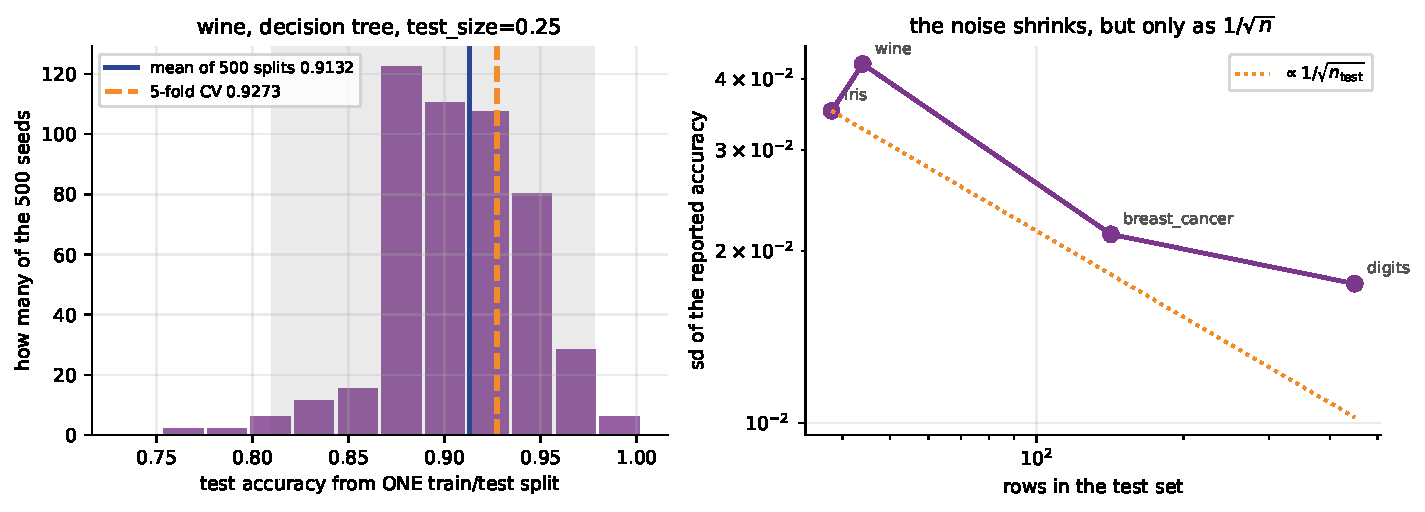
\includegraphics[width=0.88\textwidth]{splitspread.pdf}
  \caption{Left: $500$ single train/test splits of \texttt{load\_wine}, with
    the shaded band the middle $95\%$. Right: the same experiment on four
    bundled datasets. The spread falls as $1/\sqrt{n_{\text{te}}}$, so
    \emph{halving} the noise costs \emph{four times} the test set.}
  \label{fig:splitspread}
\end{figure}

\begin{lstlisting}
# fewer seeds on the bigger datasets, because each seed costs a fit
for nm, X_, y_, n in (("iris", Xi, yi, 500), ("wine", Xw, yw, 500),
                      ("breast_cancer", Xb, yb, 300), ("digits", Xg, yg, 100)):
    a = split_spread(X_, y_, DecisionTreeClassifier(random_state=0), n=n)
    print("%-14s test rows %4d   sd %.4f   min %.4f   max %.4f"
          % (nm, round(0.25*len(y_)), a.std(), a.min(), a.max()))
\end{lstlisting}
\begin{codeout}
   iris          n= 150  test rows   38   sd 0.0352   min 0.7895   max 1.0000
   wine          n= 178  test rows   44   sd 0.0425   min 0.7556   max 1.0000
   breast_cancer n= 569  test rows  142   sd 0.0214   min 0.8601   max 0.9790
   digits        n=1797  test rows  449   sd 0.0186   min 0.7800   max 0.9111
\end{codeout}

Roughly three times the test rows, roughly half the standard deviation:
$0.0425$ at $44$ rows against $0.0214$ at $142$. That is the $1/\sqrt{n}$ law,
measured.

\subsection{It is not just noisy --- it ranks models wrongly}
\label{sec:ranking}

Noise that only blurred the number would be tolerable. The real damage is that
a single split \emph{makes decisions}. Take two models that are, on average,
indistinguishable: an unpruned decision tree and the same tree limited to
depth~$3$.

\begin{lstlisting}
d = np.empty(500)
for s in range(500):
    Xtr, Xte, ytr, yte = train_test_split(Xw, yw, test_size=0.25, random_state=s)
    d[s] = (clone(m1).fit(Xtr, ytr).score(Xte, yte)      # unpruned
            - clone(m2).fit(Xtr, ytr).score(Xte, yte))   # max_depth=3
print("mean difference %+.4f  sd %.4f" % (d.mean(), d.std()))
print("depth-3 won on %d, unpruned on %d, tied on %d"
      % ((d < 0).sum(), (d > 0).sum(), (d == 0).sum()))
\end{lstlisting}
\begin{codeout}
wine: an unpruned tree against a depth-3 tree, 500 single splits
   mean difference -0.0021  sd 0.0276
   the depth-3 tree won on 119 splits, the unpruned tree on 74, tied on 307
   most extreme single-split verdicts: +0.1556 and -0.1333
\end{codeout}

\begin{caution}[If your model comparison rests on one split, you measured the split]
These two models differ by $0.0021$ on average --- two-tenths of one per cent.
A single split declared a winner on $193$ of $500$ occasions, and the size of
its verdict ranged from $+0.1556$ to $-0.1333$. Somebody who ran one seed
would write ``pruning helps by sixteen points''; somebody who ran another
would write the opposite. Both would be reporting noise with a straight face.
\end{caution}

The fix is not a luckier seed. It is to \textbf{average over many splits},
which is what the rest of this lecture is about. But before averaging, we have
to make sure the individual splits are legitimate at all.

% =========================================================================
\section{Split strategies: stratified, grouped, ordered}
\label{sec:strat}

Every random split makes one assumption:

\begin{keyidea}
Rows are \textbf{independent draws from a single population}, so any random
subset is as good as any other. When that assumption fails --- and it fails
constantly --- a random split does not merely add noise, it \emph{leaks}.
\end{keyidea}

Three failures, three repairs:

\begin{center}\small
\begin{tabular}{@{}lp{5.2cm}p{4.4cm}@{}}
  \toprule
  \textbf{When it fails} & \textbf{Why} & \textbf{What to use}\\
  \midrule
  Skewed classes & a fold may contain few or no minority rows &
    \texttt{StratifiedKFold}, \texttt{stratify=y}\\[3pt]
  Repeated measurements & rows from the same patient, sensor, image or
    customer are near-duplicates & \texttt{GroupKFold},
    \texttt{GroupShuffleSplit}, \texttt{StratifiedGroupKFold}\\[3pt]
  Time order & tomorrow is predicted from yesterday, not from next week &
    \texttt{TimeSeriesSplit}\\
  \bottomrule
\end{tabular}
\end{center}

The test that covers all three: \textbf{could a test row have been produced by
something the training set already contains?} If yes, your score measures
recall of the training set.

\subsection{Stratification, by hand and in code}
\label{sec:stratify}

Stratification is not clever. It deals each class out separately, in
proportion. On the twelve-row table of Section~\ref{sec:onesplit}, three folds:

\begin{lstlisting}
for nm, cv in (("KFold(3, shuffle=False)", KFold(3)),
               ("StratifiedKFold(3)", StratifiedKFold(3))):
    for k, (tr, te) in enumerate(cv.split(X12, y12)):
        print("fold %d  test rows %s  y %s  minority %d"
              % (k+1, te.tolist(), y12[te].tolist(), y12[te].sum()))
\end{lstlisting}
\begin{codeout}
twelve rows, y = [0, 0, 0, 0, 0, 0, 0, 0, 0, 1, 1, 1]
   KFold(3, shuffle=False)
      fold 1  test rows [0, 1, 2, 3]    y [0, 0, 0, 0]  minority 0
      fold 2  test rows [4, 5, 6, 7]    y [0, 0, 0, 0]  minority 0
      fold 3  test rows [8, 9, 10, 11]  y [0, 1, 1, 1]  minority 3
   StratifiedKFold(3)
      fold 1  test rows [0, 1, 2, 9]    y [0, 0, 0, 1]  minority 1
      fold 2  test rows [3, 4, 5, 10]   y [0, 0, 0, 1]  minority 1
      fold 3  test rows [6, 7, 8, 11]   y [0, 0, 0, 1]  minority 1
\end{codeout}

Three ill patients, three folds, one each: exactly the arithmetic of the
worked example. Note also that \texttt{KFold} \emph{without} \texttt{shuffle}
takes contiguous blocks of rows, which on a sorted file is the worst available
choice --- and \texttt{shuffle=False} is the default.

\subsection{A fold with nothing to learn from}

Scale it up: $200$ rows, $10$ positives ($5\%$), file sorted by label.

\begin{lstlisting}
for nm, cv in (("KFold(5, shuffle=False)", KFold(5)),
               ("KFold(5, shuffle=True, random_state=0)",
                KFold(5, shuffle=True, random_state=0)),
               ("StratifiedKFold(5, shuffle=True, random_state=0)",
                StratifiedKFold(5, shuffle=True, random_state=0))):
    print("%-48s positives per test fold %s"
          % (nm, [int(y_im[te].sum()) for _, te in cv.split(X_im, y_im)]))
\end{lstlisting}
\begin{codeout}
200 rows, 10 positives (5%), and the file is sorted by label
   KFold(5, shuffle=False)                          positives per test fold [10, 0, 0, 0, 0]
   KFold(5, shuffle=True, random_state=0)           positives per test fold [3, 1, 2, 3, 1]
   StratifiedKFold(5, shuffle=True, random_state=0) positives per test fold [2, 2, 2, 2, 2]
\end{codeout}

Look at what \texttt{KFold(5, shuffle=False)} has done, in class counts:

\begin{codeout}
KFold(5, shuffle=False) class counts, [negatives positives]:
   fold 1  train [160, 0]   test [30, 10]
   fold 2  train [150, 10]   test [40, 0]
   fold 3  train [150, 10]   test [40, 0]
   fold 4  train [150, 10]   test [40, 0]
   fold 5  train [150, 10]   test [40, 0]
\end{codeout}

Fold~1's \emph{training set contains one class}. A classifier cannot be fitted
at all, so scikit-learn returns \texttt{nan} for that fold. Folds $2$--$5$
contain no positives to test on, so each of them scores accuracy $1.0000$ and
recall $0$ vacuously. Cross-validate and read the summary:

\begin{codeout}
   KFold(5, shuffle=False)          recall   per fold [nan, 0.0, 0.0, 0.0, 0.0]
                                    accuracy per fold [nan, 1.0, 1.0, 1.0, 1.0]
                                    mean recall 0.0000   mean accuracy 1.0000
   KFold(5, shuffle=True)           recall   per fold [0.6667, 1.0, 0.5, 0.3333, 1.0]
                                    accuracy per fold [0.975, 1.0, 0.975, 0.95, 1.0]
                                    mean recall 0.7000   mean accuracy 0.9800
   StratifiedKFold(5, shuffle=True) recall   per fold [1.0, 0.5, 0.5, 0.5, 0.5]
                                    accuracy per fold [1.0, 0.975, 0.975, 0.975, 0.975]
                                    mean recall 0.6000   mean accuracy 0.9800
\end{codeout}

\begin{caution}[Mean accuracy $1.0000$, mean recall $0.0000$, and no error message]
The first row is a perfect score produced by a broken experiment. Nothing in
the output says so. The only defence is to look at the per-fold numbers and
the per-fold class counts --- not the mean.
\end{caution}

Notice a second, subtler point in that table. Shuffling repaired the
catastrophe but gave folds with $1$, $2$ and $3$ positives, and the mean
recall it reports ($0.7000$) is \emph{higher} than the stratified one
($0.6000$). Higher is not better here: it is an average over folds of unequal
difficulty. On the three-class wine data the same effect shows up as a drift
in the class mix:

\begin{codeout}
   KFold(5, shuffle=True, random_state=0)
      class 0 share per fold [0.3889, 0.2222, 0.3333, 0.4286, 0.2857]
      largest deviation from the overall share 0.1132
   StratifiedKFold(5, shuffle=True, random_state=0)
      class 0 share per fold [0.3333, 0.3333, 0.3333, 0.3429, 0.3143]
      largest deviation from the overall share 0.0297
   overall class shares [0.3315, 0.3989, 0.2697]
\end{codeout}

\begin{figure}[htbp]
  \centering
  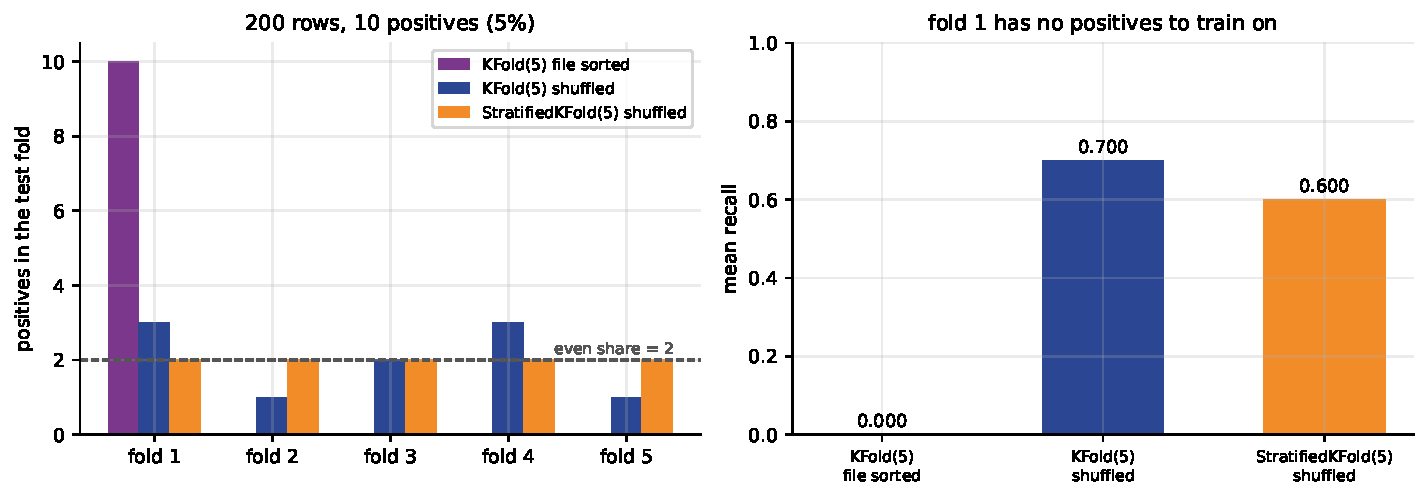
\includegraphics[width=0.86\textwidth]{stratify.pdf}
  \caption{A $5\%$ minority in a sorted file. Left: positives per test fold
    under three splitters. Right: the mean recall each one reports ---
    $0.000$, $0.700$, $0.600$. Stratifying gives the \emph{lowest} number of
    the three and the only trustworthy one.}
  \label{fig:stratify}
\end{figure}

\begin{keyidea}
For classification, stratify by default. \texttt{cross\_val\_score} already
does when you pass an integer \texttt{cv} and a classifier; if you construct
the splitter yourself, construct
\texttt{StratifiedKFold(k, shuffle=True, random\_state=...)}, not
\texttt{KFold(k)}.
\end{keyidea}

\subsection{Grouped rows: the unit of independence}
\label{sec:groups}

Here is the experiment that convinces people. Forty patients. Each contributes
fifteen windows of a recorded signal, so $600$ rows. Each patient's
\textbf{diagnosis is a coin flip}, unrelated to anything. Each patient has a
random ten-dimensional ``fingerprint'' --- a baseline that says nothing about
the diagnosis --- and the features are that fingerprint plus noise.

There is nothing to learn. The honest score is $0.5000$.

\begin{lstlisting}
pat_sig = rng.normal(size=(40, 10)) * 2.0      # a per-patient fingerprint
y_pat   = rng.integers(0, 2, 40)               # diagnosis: a coin flip
groups  = np.repeat(np.arange(40), 15)
Xp = pat_sig[groups] + rng.normal(size=(600, 10)) * 0.5
yp = y_pat[groups]

knn = make_pipeline(StandardScaler(), KNeighborsClassifier(5))
print(cross_val_score(knn, Xp, yp,
                      cv=StratifiedKFold(5, shuffle=True, random_state=0)).mean())
print(cross_val_score(knn, Xp, yp, groups=groups, cv=GroupKFold(5)).mean())
\end{lstlisting}
\begin{codeout}
   random 5-fold, rows shuffled : 1.0000  +/- 0.0000
   GroupKFold(5) by patient     : 0.6483  +/- 0.1984
   overstatement                : +0.3517
   patients in BOTH train and test, random fold 1  : 37 of 40
   patients in BOTH train and test, GroupKFold fold 1: 0
\end{codeout}

$\mathbf{1.0000 \pm 0.0000}$ on a coin flip. Thirty-seven of the forty
patients had windows on both sides of fold~1, so the nearest neighbour of a
test window was another window \emph{from the same patient}, and the model
simply read the label off it. The classifier is not diagnosing; it is
recognising.

Two further things to read in that output. First, \texttt{GroupKFold} gives
$0.6483$, not $0.5000$ --- with only forty independent patients, an estimate
of a coin flip is itself noisy. Second, and more important, the honest
estimate comes with an honest error bar, $\pm 0.1984$, because you have
\textbf{forty} independent observations and not six hundred. The random split
reported no uncertainty at all, which should always be the first thing you
distrust.

\begin{figure}[htbp]
  \centering
  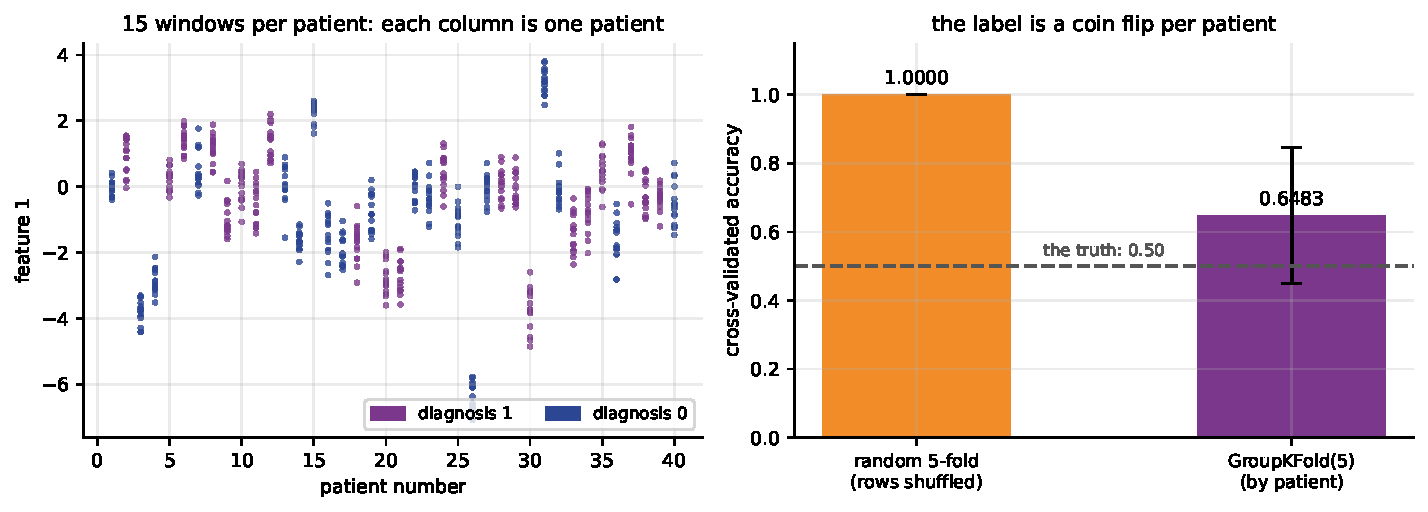
\includegraphics[width=0.86\textwidth]{groups.pdf}
  \caption{Left: each cluster is one patient's fifteen windows, projected onto
    two dimensions --- tight, and all carrying the same label. Right: the two
    verdicts on the same data.}
  \label{fig:groups}
\end{figure}

\begin{keyidea}
Ask ``what is the unit of independence?'' before you split. It is the patient,
not the window; the customer, not the transaction; the document, not the
sentence; the subject, not the trial.
\end{keyidea}

\begin{caution}[Grouping is not the same as stratifying, and you often need both]
\texttt{GroupKFold} keeps groups intact but ignores the class balance;
\texttt{StratifiedKFold} balances classes but ignores groups. When the target
is skewed \emph{and} the rows are grouped, use \texttt{StratifiedGroupKFold},
which attempts both. Note also that \texttt{GroupKFold} is deterministic: to
average over several groupings, use \texttt{GroupShuffleSplit} with different
seeds.
\end{caution}

\subsection{Time-ordered rows}
\label{sec:time}

Six hundred days of a drifting, seasonal series: a random walk, plus a linear
trend, plus a $30$-day seasonal cycle, plus noise. The features are the day
index and two seasonal terms; the model is a random forest.

\begin{lstlisting}
itr, ite = train_test_split(np.arange(600), test_size=0.25, random_state=0)
r_shuf = clone(rf).fit(Xt[itr], series[itr]).score(Xt[ite], series[ite])
cut = 450
r_time = clone(rf).fit(Xt[:cut], series[:cut]).score(Xt[cut:], series[cut:])
r_tss  = cross_val_score(rf, Xt, series, cv=TimeSeriesSplit(5), scoring="r2")
\end{lstlisting}
\begin{codeout}
600 days of a drifting seasonal series; the features are the day
index and two seasonal terms
   random 75/25 split               R2 +0.9975
   train on the first 75% of days   R2 -2.7683
   TimeSeriesSplit(5), per fold     [-1.8789, -0.0513, 0.0816, -4.1669, -8.0681]
   TimeSeriesSplit(5), mean         R2 -2.8167
   overstatement from shuffling     +3.8142
   in the random split the median gap between consecutive TRAINING
   days is 1: almost every test day sits between two training days
   92 of the 150 test days have BOTH neighbours in the training set (61.3%)
\end{codeout}

$R^2 = +0.9975$ against an honest $-2.8167$. This is the most persuasive
failure in the lecture, and the mechanism is visible in the last two lines: a
random split leaves $61.3\%$ of test days with \emph{both} neighbours in the
training set, so the model interpolates between two known values. In
production it must \textbf{extrapolate}, and a random forest structurally
cannot: every prediction it makes is an average of training targets, so it is
bounded by the range of the training targets. When the series keeps climbing,
the forest's prediction flattens.

Remember what a negative $R^2$ means: \textbf{you would have done better
predicting the training mean for every day}.

\begin{figure}[htbp]
  \centering
  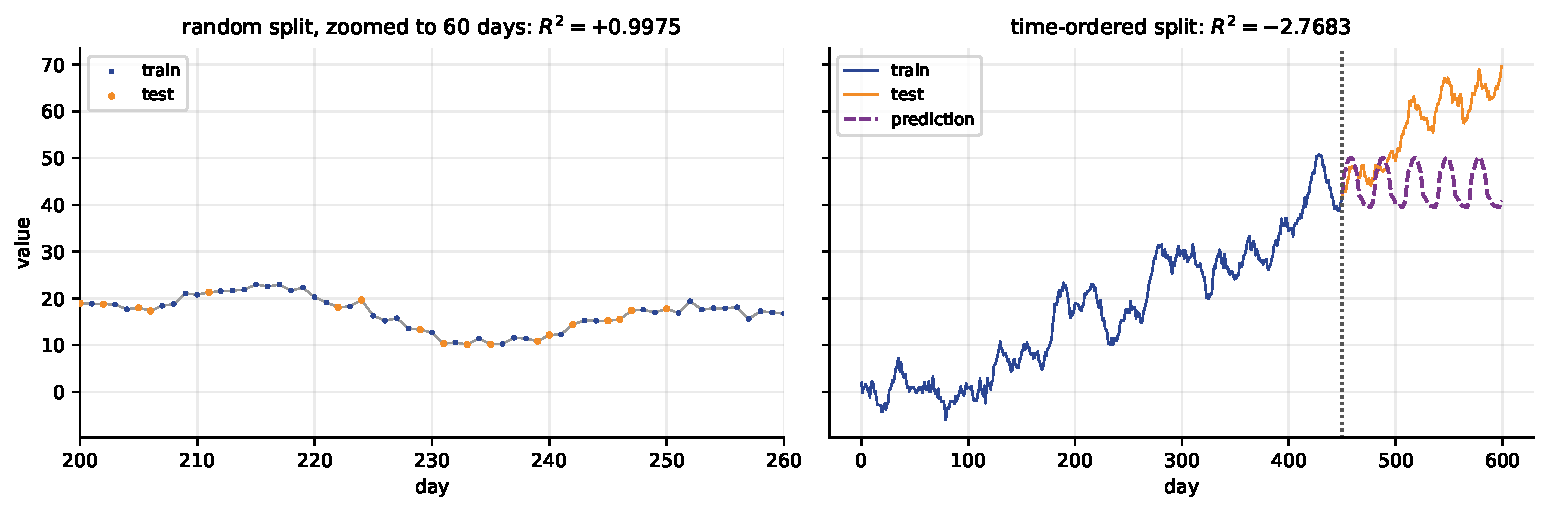
\includegraphics[width=0.88\textwidth]{timeseries.pdf}
  \caption{Left, zoomed to sixty days: orange test points sitting between blue
    training points --- the interpolation the random split rewards. Right:
    trained on the first $450$ days, the forest's prediction flattens the
    moment it leaves the training range.}
  \label{fig:timeseries}
\end{figure}

\texttt{TimeSeriesSplit(k)} produces $k$ folds in which the training set is
always a prefix of the series and the test set is the block immediately after
it. The training set grows from fold to fold; no fold ever trains on the
future.

The damage is not confined to the number. Compare two candidate models on the
same $600$ days --- (A) calendar features with a random forest, (B) yesterday's
value and a trailing mean with a linear model:

\begin{codeout}
   A: calendar features + random forest  shuffled 5-fold R2 +0.9974   TimeSeriesSplit R2 -2.8167
   B: lag-1 + trailing mean + linear     shuffled 5-fold R2 +0.9967   TimeSeriesSplit R2 +0.9230
   shuffled cross-validation ranks A above B and would ship A.
   A cannot extrapolate past the training range at all.
\end{codeout}

\begin{caution}[The wrong splitter inverts the decision, not just the number]
On the shuffled evidence, $0.9974$ beats $0.9967$ and you ship model A. In
time order, A scores $-2.82$ and B scores $+0.92$. The splitter did not merely
inflate a score; it reversed the choice the score existed to make.
\end{caution}

\begin{figure}[htbp]
  \centering
  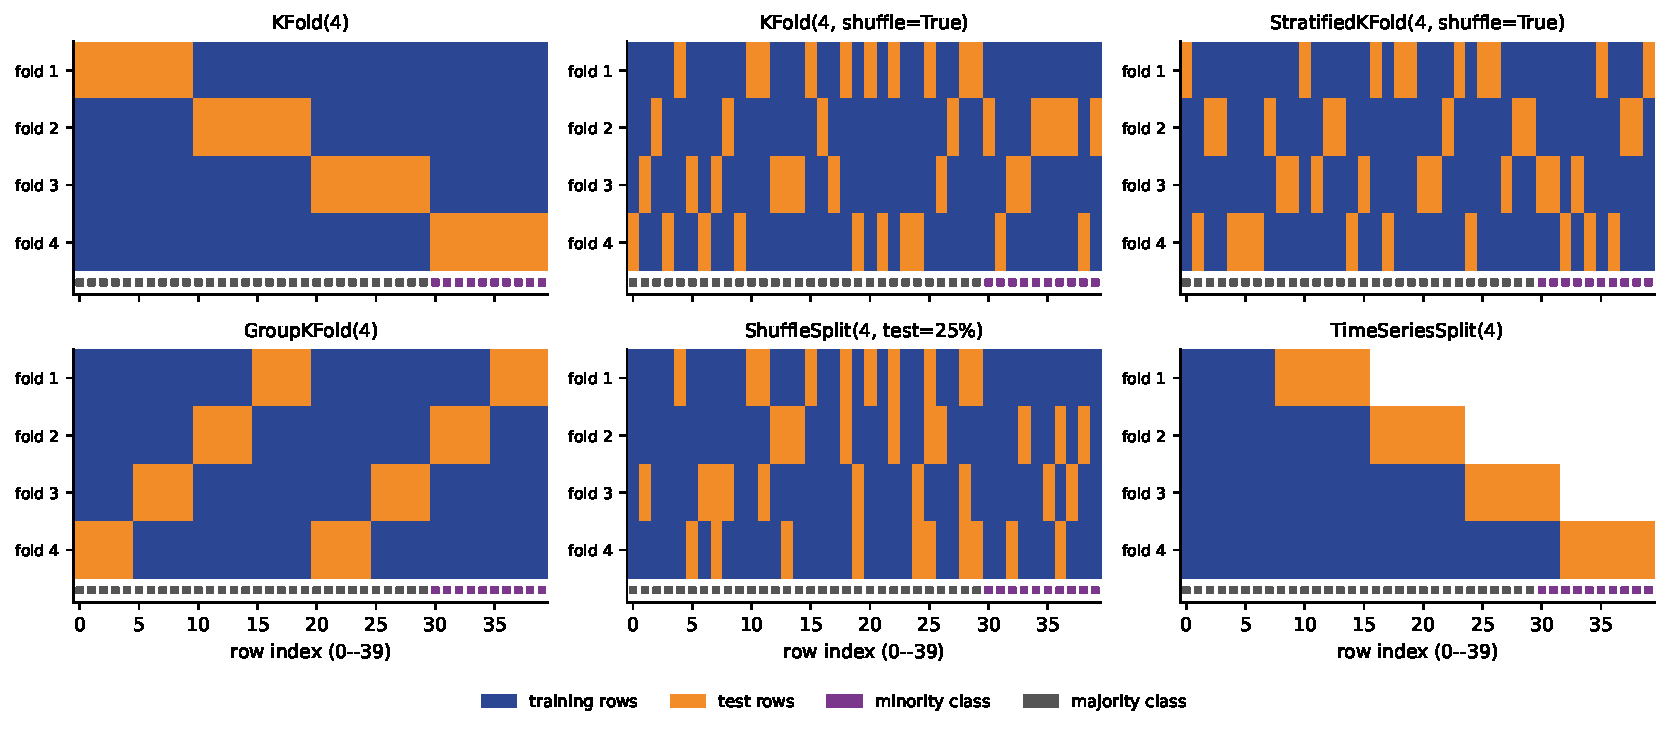
\includegraphics[width=0.88\textwidth]{cvsplits.pdf}
  \caption{Six splitters on the same forty rows --- ten of them minority,
    arriving sorted, in eight groups of five. Every band was drawn from the
    indices the splitter actually returned. Minority rows per test fold:
    \texttt{KFold} $[0,0,0,10]$; shuffled $[0,6,2,2]$; stratified
    $[2,2,3,3]$; \texttt{GroupKFold} $[5,5,0,0]$; \texttt{TimeSeriesSplit}
    $[0,0,2,8]$.}
  \label{fig:cvsplits}
\end{figure}

\begin{tryit}[Draw your own splitter]
Take any \texttt{cv} object and print what it actually does:
\begin{lstlisting}
for k, (tr, te) in enumerate(TimeSeriesSplit(4).split(np.zeros((40, 1)))):
    print(k, "train", len(tr), "test", te[:3], "...", te[-1])
\end{lstlisting}
Expected: training sets of size $8, 16, 24, 32$ and test blocks of $8$ that
never precede their training set. Two minutes of this will tell you more than
any diagram --- including whether your own data really is grouped.
\end{tryit}

% =========================================================================
\section{Cross-validation}
\label{sec:cv}

\subsection{The recipe, and its cost}

$k$-fold cross-validation:

\begin{enumerate}[leftmargin=*]
  \item Cut the rows into $k$ folds.
  \item For each fold in turn: train on the other $k-1$ folds, test on this
    one.
  \item Report the \textbf{mean} of the $k$ scores --- and the \textbf{spread}.
\end{enumerate}

Every row is tested exactly once, so the estimate is built from all $n$ rows
rather than from $n/4$; and you get $k$ numbers instead of one, so you can see
how variable the answer is.

\begin{worked}[The cost model, on $n = 5000$ rows]
\begin{center}\small
\begin{tabular}{@{}lrrr@{}}
  \toprule
  & fits & rows per fit & row-fits\\
  \midrule
  $2$-fold  & $2$ & $2500$ & $5{,}000$\\
  $5$-fold  & $5$ & $4000$ & $20{,}000$\\
  $10$-fold & $10$ & $4500$ & $45{,}000$\\
  LOOCV     & $5000$ & $4999$ & $24{,}995{,}000$\\
  \bottomrule
\end{tabular}
\end{center}
$k$-fold costs $k$ times one fit --- that is the whole cost model. The
row-fits column is $k \cdot n(1 - 1/k) = n(k-1)$, linear in $k$, so LOOCV is
about $n$ times the work of a single fit on almost all the data.
\end{worked}

\subsection{Choosing $k$: bias, variance and time}
\label{sec:kchoice}

Three things change as $k$ grows. Measure all three on
\texttt{load\_breast\_cancer} with a scaler and a logistic regression.

\begin{lstlisting}
PIPE = make_pipeline(StandardScaler(), LogisticRegression(max_iter=5000))
for nm, cv, nfit in (("2-fold", StratifiedKFold(2, shuffle=True, random_state=0), 2),
                     ...,
                     ("LOOCV", LeaveOneOut(), len(yb))):
    t0 = time.perf_counter()
    s = cross_val_score(PIPE, Xb, yb, cv=cv)
    print("%s %4d fits  trains on %3d rows  accuracy %.4f  %6.2f s"
          % (nm, nfit, len(yb)*(1 - 1/nfit), s.mean(), time.perf_counter()-t0))
\end{lstlisting}
\begin{codeout}
   2-fold      2 fits   trains on 284 rows   accuracy 0.9859     0.01 s
   5-fold      5 fits   trains on 455 rows   accuracy 0.9789     0.01 s
   10-fold    10 fits   trains on 512 rows   accuracy 0.9772     0.03 s
   20-fold    20 fits   trains on 540 rows   accuracy 0.9790     0.06 s
   LOOCV     569 fits   trains on 568 rows   accuracy 0.9789     1.62 s
   LOOCV fits the model 569 times against 5-fold's 5: 113.8 times as many,
   and that ratio is the same on every machine
   on this run the wall clock made it 112 times, but the seconds above are
   a measurement, not a reproducible number
   sd ACROSS FOLDS: 5-fold 0.0142   LOOCV 0.1437  <- not comparable
\end{codeout}

\textbf{Bias.} Read the third column, not the fifth. $2$-fold trains each
model on $284$ rows; $20$-fold trains it on $540$. A model trained on fewer
rows is worse, so small $k$ \emph{underestimates} the performance of the model
you will actually ship, which is trained on everything. That is the bias of
$k$-fold, and its size is the slope of the learning curve:

\begin{codeout}
bias: what a smaller training set costs
   train on  50 rows  ->  held-out accuracy 0.9566
   train on 100 rows  ->  held-out accuracy 0.9666
   train on 200 rows  ->  held-out accuracy 0.9709
   train on 300 rows  ->  held-out accuracy 0.9749
   train on 400 rows  ->  held-out accuracy 0.9757
   train on 455 rows  ->  held-out accuracy 0.9741
   train on 512 rows  ->  held-out accuracy 0.9763
   train on 540 rows  ->  held-out accuracy 0.9776
\end{codeout}

Between $455$ rows (what $5$-fold trains on) and $540$ rows (what $20$-fold
trains on) the curve moves by about $0.003$. On this dataset the bias of
$5$-fold is therefore small, because $569$ rows is already past the steep part
of the curve. On $60$ rows it would not be: from $50$ to $100$ rows the curve
moves by $0.010$, three times as much.

\textbf{Cost.} Read the second column, not the fifth. The cost of $k$-fold is
$k$ fits of the model, so LOOCV on these $569$ rows costs $569$ fits against
$5$-fold's $5$: \textbf{$113.8$ times as many, for an identical answer of
$0.9789$}. That ratio is arithmetic and it is the same on your machine as on
mine.

\begin{caution}[The seconds are a measurement; the fits are the claim]
The last column of that table is the one thing in these notes that will not
reproduce. It depends on your processor, your BLAS build and what else is
running, and it varies between runs \emph{on the same machine}: repeated runs
of exactly this comparison gave LOOCV/$5$-fold wall-clock ratios of $112$,
$122$, $126$ and $131$ while the fit ratio stayed at $113.8$ throughout.

So quote the fits and never the seconds. If you time it and get a different
ratio, you are not wrong --- and neither is the person next to you who got
another one. When you need a defensible cost claim, count model fits.
\end{caution}

\begin{caution}[\texttt{cross\_val\_score(...).std()} is not the uncertainty of the mean]
In the table above, the across-fold sd is $0.0142$ for $5$-fold and $0.1437$
for LOOCV. That does \emph{not} mean LOOCV is ten times less stable. Each
LOOCV fold scores a single row, so its score is $0$ or $1$ and the across-fold
sd is just $\sqrt{p(1-p)} \approx \sqrt{0.979 \times 0.021} = 0.143$. It is a
property of the scoring, not of the estimator. The quantity you actually care
about is the spread of the \emph{mean}, which needs repetition to measure.
\end{caution}

\subsection{Variance of the estimate, measured properly}

Repeat the whole cross-validation with $40$ different shuffles and look at how
much the reported mean moves.

\begin{lstlisting}
for k in (2, 5, 10, 20):
    means = np.array([cross_val_score(
        PIPE, Xb, yb,
        cv=StratifiedKFold(k, shuffle=True, random_state=s)).mean()
        for s in range(40)])
    print("%2d-fold  mean of means %.4f  sd of the mean %.4f  range %.4f"
          % (k, means.mean(), means.std(), means.max() - means.min()))
\end{lstlisting}
\begin{codeout}
spread of the cross-validated MEAN over 40 different shuffles
    2-fold   mean of means 0.9754   sd of the mean 0.0042   range 0.0194
    5-fold   mean of means 0.9782   sd of the mean 0.0030   range 0.0123
   10-fold   mean of means 0.9786   sd of the mean 0.0025   range 0.0106
   20-fold   mean of means 0.9791   sd of the mean 0.0019   range 0.0072
   LOOCV     mean          0.9789   sd of the mean 0.0000   (no shuffle: LOOCV is deterministic)
   one 80/20 split, 40 seeds: mean 0.9772   sd 0.0114   range 0.0526
\end{codeout}

Two results, one of them uncomfortable.

The comfortable one: \textbf{cross-validation is about four times steadier
than a single split}, for five times the compute. $5$-fold has sd $0.0030$
where one $80/20$ split has $0.0114$.

The uncomfortable one: on this dataset the variance \emph{falls} as $k$ rises,
and LOOCV has none at all --- it does not shuffle, so re-running it changes
nothing. Textbooks routinely say ``LOOCV has high variance''. That claim is
about the variance across \emph{different datasets} drawn from the same
population, driven by the near-total overlap of LOOCV's training sets, and it
is not what this experiment measures. Report the experiment you ran, not the
one the textbook predicted. What LOOCV certainly is here is a hundred times
slower for the same answer.

\begin{figure}[htbp]
  \centering
  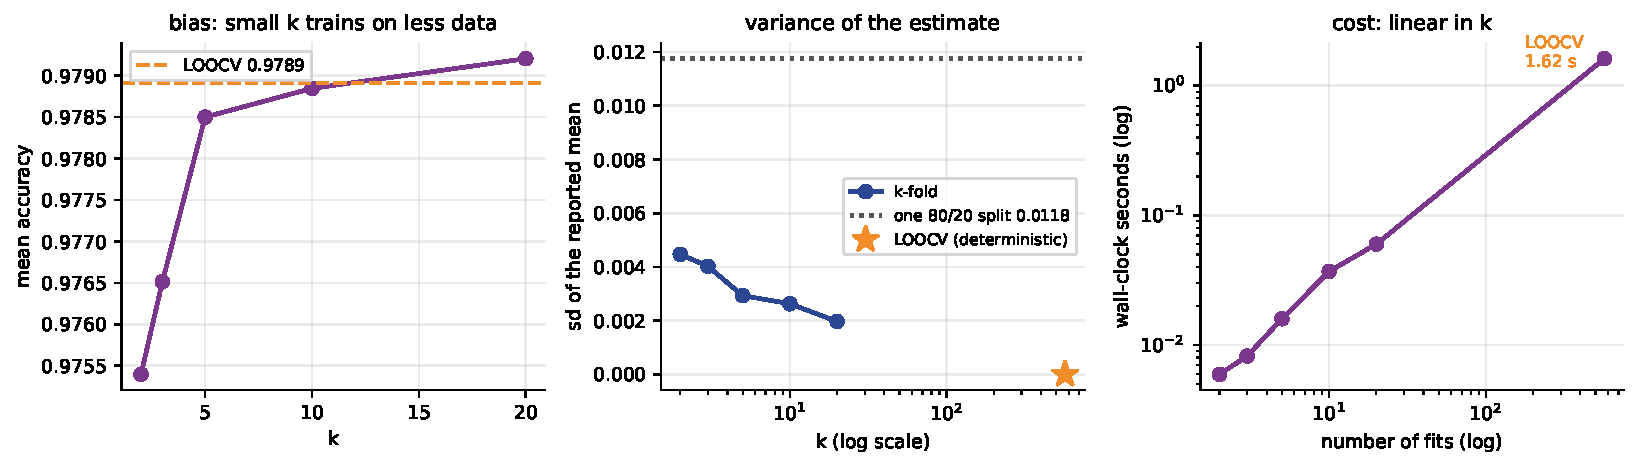
\includegraphics[width=0.90\textwidth]{kchoice.pdf}
  \caption{Left: the estimate rises with $k$ and flattens --- the bias going
    away. Middle: the spread of the estimate falls with $k$; the dotted line
    is a single $80/20$ split. Right: cost is exactly linear in the number of
    fits. Five or ten folds is where the three curves meet.}
  \label{fig:kchoice}
\end{figure}

\begin{keyidea}
Use $k = 5$ or $k = 10$. Use more folds when $n$ is small and a fit is cheap;
use fewer when a fit is expensive. Do not use LOOCV because it sounds
thorough.
\end{keyidea}

\subsection{More folds, or more repeats?}

If $5$-fold is still too wobbly, you can repeat it with different shuffles
rather than increasing $k$.

\begin{codeout}
   StratifiedKFold(5)                       5 fits  accuracy 0.9789 +/- 0.0142    0.02 s
   RepeatedStratifiedKFold(5 x 10)         50 fits  accuracy 0.9772 +/- 0.0147    0.18 s
   StratifiedShuffleSplit(50, test 20%)    50 fits  accuracy 0.9767 +/- 0.0122    0.17 s
\end{codeout}

\begin{center}\small
\begin{tabular}{@{}lp{9.4cm}@{}}
  \toprule
  \texttt{StratifiedKFold(5)} & the default for classification. Use it.\\
  \texttt{KFold(5, shuffle=True)} & regression, or classification with a
    balanced target.\\
  \texttt{RepeatedStratifiedKFold} & when $n$ is small and you need the
    estimate to stop wobbling before you can compare two models.\\
  \texttt{ShuffleSplit}, \texttt{StratifiedShuffleSplit} & when you want the
    test size and the number of repeats to be independent of each other. Rows
    may appear in several test sets, and some in none.\\
  \texttt{LeaveOneOut} & when $n$ is tiny and a fit is cheap.\\
  \texttt{GroupKFold}, \texttt{StratifiedGroupKFold},
    \texttt{TimeSeriesSplit} & whenever the rows are not independent.
    \textbf{Not optional.}\\
  \bottomrule
\end{tabular}
\end{center}

\begin{tryit}[Report a score the way a reviewer will accept]
\begin{lstlisting}
cv = StratifiedKFold(5, shuffle=True, random_state=0)
s = cross_val_score(PIPE, Xb, yb, cv=cv)
print("accuracy %.4f +/- %.4f over %d folds" % (s.mean(), s.std(), len(s)))
\end{lstlisting}
Expected: \texttt{accuracy 0.9789 +/- 0.0142 over 5 folds}. Never report the
first number without the second, and never report either without saying which
splitter produced them.
\end{tryit}

% =========================================================================
\section{Tuning honestly: validation sets and nested CV}
\label{sec:nested}

\subsection{The moment you tune, the score stops being an estimate}

Split breast\_cancer three ways --- train, validation, test --- and choose $C$
for a logistic regression on the validation set.

\begin{codeout}
the three-way split, done once, on breast_cancer
   train 341   validation 114   test 114
      C=  0.01  validation 0.9561
      C=  0.10  validation 0.9561
      C=  1.00  validation 0.9474
      C= 10.00  validation 0.9474
      C=100.00  validation 0.9298
   chosen C=0.01   validation 0.9561   TEST 0.9386
\end{codeout}

$0.9561$ is the \emph{maximum of five noisy numbers}. It is biased upward by
construction, for the same reason that the tallest of five randomly chosen
people is taller than average. $0.9386$ is the estimate.

\begin{keyidea}
The validation set \textbf{selects}. The test set \textbf{estimates}. A number
that was used to choose something can never also be the estimate of what was
chosen --- and you may look at the test set once.
\end{keyidea}

\subsection{Predict the number first: tuning on pure noise}
\label{sec:noise}

Cross-validation replaces the validation \emph{set}, but it does not remove
the need for a validation \emph{step}. If the tuning happens inside the same
folds you report, the bias comes straight back. Here is how much.

One hundred rows, two hundred features, everything drawn from
$\mathcal{N}(0,1)$. The labels are coin flips --- fifty zeros and fifty ones,
permuted. \textbf{There is no signal whatsoever; the truth is $0.5000$.} Tune
an RBF SVM over five values of $C$ and four of $\gamma$ with $5$-fold
cross-validation, and report \texttt{GridSearchCV.best\_score\_}.

Write down what you expect before reading on.

\begin{lstlisting}
def nested_experiment(X, y, grid, est, trials=20, inner=5, outer=5):
    non_nested, nested = [], []
    for t in range(trials):
        icv = StratifiedKFold(inner, shuffle=True, random_state=t)
        ocv = StratifiedKFold(outer, shuffle=True, random_state=t)
        gs = GridSearchCV(est, grid, cv=icv).fit(X, y)
        non_nested.append(gs.best_score_)                       # the wrong way
        nested.append(cross_val_score(GridSearchCV(est, grid, cv=icv),
                                      X, y, cv=ocv).mean())     # the right way
    return np.array(non_nested), np.array(nested)
\end{lstlisting}
\begin{codeout}
pure noise, 100 rows x 200 features, coin-flip labels (the truth is 0.5000)
   tune and report on the SAME folds : 0.5820  +/- 0.0314
   nested cross-validation           : 0.5265  +/- 0.0419
   optimism                          : +0.0555
   the wrong way beat 0.5 on 20 of 20 trials
   grid: 20 combinations, so 100 inner fits per trial
\end{codeout}

Eight points of accuracy above the truth, conjured out of nothing, on twenty
trials out of twenty. The mechanism is not subtle: \texttt{best\_score\_} is
the \textbf{maximum} of twenty cross-validated numbers, each carrying a
standard error of a few points, and the maximum of twenty noisy numbers is
larger than their mean. If each of $m$ combinations has true score $\mu$ and
independent noise of sd $\sigma$, the expected maximum is roughly
$\mu + \sigma \sqrt{2 \ln m}$ --- it grows with the size of the grid, slowly
but without limit.

\begin{caution}[\texttt{best\_score\_} is a selection, not an estimate]
It is the score of the winner, measured on the same folds that crowned it. It
must never be reported as performance. Report either a nested
cross-validation, or the score of the tuned model on a test set that the
search never touched.
\end{caution}

\subsection{The same effect where there is real signal}

Noise is a demonstration; here is the everyday case. A $120$-row subsample of
breast\_cancer --- real signal, real structure --- with the same grid and
twenty trials.

\begin{codeout}
breast_cancer, a 120-row subsample -- real signal this time
   tune and report on the SAME folds : 0.9529  +/- 0.0054
   nested cross-validation           : 0.9317  +/- 0.0094
   optimism                          : +0.0212
   paired t over 20 trials: t = 9.58, p = 1.1e-08
   the wrong way was higher on 19 of 20 trials
\end{codeout}

Two points of accuracy --- and two points is very often the entire claimed
improvement in a student project. The paired $t$-test over the twenty trials
gives $p = 1.1 \times 10^{-8}$: this is a systematic bias, not a run of luck.

And the size of the bias is set by how hard you searched:

\begin{codeout}
the more hyper-parameter combinations you try, the luckier you get
(pure noise again, so every one of these should be 0.5000)
    1 combinations   same-fold 0.5467   nested 0.5467   optimism +0.0000
    4 combinations   same-fold 0.5767   nested 0.5567   optimism +0.0200
   20 combinations   same-fold 0.5833   nested 0.5217   optimism +0.0617
   60 combinations   same-fold 0.5850   nested 0.5067   optimism +0.0783
\end{codeout}

The first row is the proof of the mechanism. With one combination in the grid
there is nothing to choose between, so there is nothing to over-fit, and the
optimism is \textbf{exactly zero} --- the two numbers are identical to four
decimal places. Every point of optimism in the rows below it is the price of
the search.

\begin{figure}[htbp]
  \centering
  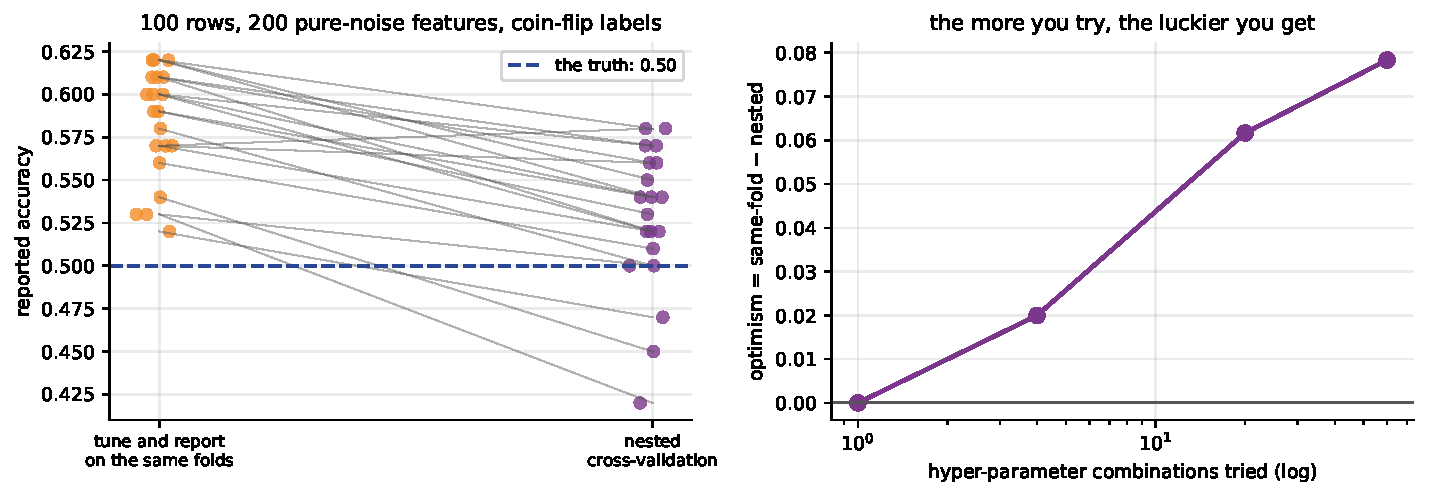
\includegraphics[width=0.86\textwidth]{nested.pdf}
  \caption{Left: twenty paired trials on pure noise; each grey line joins one
    trial's two estimates. Every same-fold point is above $0.50$; the nested
    points scatter around it as they should. Right: optimism against grid
    size, from $+0.0000$ at one combination to $+0.0783$ at sixty.}
  \label{fig:nested}
\end{figure}

\subsection{Nested cross-validation}

\begin{lstlisting}
inner = StratifiedKFold(5, shuffle=True, random_state=0)
outer = StratifiedKFold(5, shuffle=True, random_state=0)
search = GridSearchCV(pipe, grid, cv=inner)        # chooses hyper-parameters
score  = cross_val_score(search, X, y, cv=outer)   # estimates performance
print("%.4f +/- %.4f" % (score.mean(), score.std()))
\end{lstlisting}

The inner loop \textbf{selects}; the outer loop \textbf{estimates}. The outer
test fold is never involved in choosing anything: not the scaler's mean, not
the feature subset, not $C$, not $\gamma$. Each outer fold may choose a
different $C$, and that is correct --- what you are estimating is the
performance of \emph{the whole procedure}, tuning included, not of one
particular $C$.

\begin{worked}[What nested CV costs, and when it is worth it]
With a $20$-point grid, $5$ inner folds and $5$ outer folds, one nested
estimate costs $5 \times 5 \times 20 = 500$ fits, against $100$ for a plain
\texttt{GridSearchCV}. Five times the compute.

Use nested CV when the number you are about to write down is a
\textbf{performance claim}. Use plain \texttt{GridSearchCV} when you are
\textbf{choosing a model} and will evaluate the winner later on a held-out
test set. Both are correct. Quoting \texttt{best\_score\_} as your result is
not.
\end{worked}

% =========================================================================
\section{Imbalanced data}
\label{sec:imbal}

\subsection{By hand: one thousand patients, ten of them ill}

A model that always answers ``healthy'':

\begin{center}\small
\begin{tabular}{@{}lcc@{}}
  \toprule
  & predicted healthy & predicted ill\\
  \midrule
  actually healthy & $\mathrm{TN} = 990$ & $\mathrm{FP} = 0$\\
  actually ill     & $\mathrm{FN} = 10$  & $\mathrm{TP} = 0$\\
  \bottomrule
\end{tabular}
\end{center}

\begin{worked}[The four numbers]
\begin{align*}
  \text{accuracy}  &= \frac{\mathrm{TP} + \mathrm{TN}}
     {\mathrm{TP}+\mathrm{TN}+\mathrm{FP}+\mathrm{FN}}
     = \frac{0 + 990}{1000} = \mathbf{0.990},\\
  \text{recall}    &= \frac{\mathrm{TP}}{\mathrm{TP}+\mathrm{FN}}
     = \frac{0}{0+10} = \mathbf{0},\\
  \text{precision} &= \frac{\mathrm{TP}}{\mathrm{TP}+\mathrm{FP}}
     = \frac{0}{0} \quad \text{undefined (reported as 0)},\\
  \text{balanced accuracy} &= \tfrac12\!\left(\frac{\mathrm{TN}}
     {\mathrm{TN}+\mathrm{FP}} + \frac{\mathrm{TP}}{\mathrm{TP}+\mathrm{FN}}
     \right) = \tfrac12(1 + 0) = \mathbf{0.500}.
\end{align*}
Ninety-nine per cent accurate, and it has never once found an ill patient.
When $\mathrm{TN}$ is $99\%$ of the table, accuracy is a report on
$\mathrm{TN}$.
\end{worked}

\begin{keyidea}
\textbf{Recall} asks about the row you care about --- of the ill patients, how
many did we find? \textbf{Precision} asks about the column you act on --- of
the people we called ill, how many were? $F_1$ is their harmonic mean.
\textbf{PR-AUC} (average precision) summarises the whole precision--recall
curve, and its chance baseline is the positive rate, not $0.5$.
\end{keyidea}

\subsection{The same thing measured}

Five thousand rows, fifty positives ($1\%$), twenty features of which six are
informative.

\begin{codeout}
make_classification: 5000 rows, 50 positives (1.00%), ratio 99:1
   DummyClassifier(most_frequent) -- it always says 'negative'
      accuracy  0.9900
      precision 0.0000   recall 0.0000   F1 0.0000
      balanced accuracy 0.5000   PR-AUC 0.0100
      confusion matrix [[TN FP][FN TP]] = [[1485, 0], [15, 0]]
\end{codeout}

Now a real logistic regression on the same split:

\begin{codeout}
   plain LogisticRegression on the same split
      accuracy  0.9867  (the dummy got 0.9900)
      precision 0.0000   recall 0.0000   F1 0.0000
      balanced accuracy 0.4983   ROC-AUC 0.8553   PR-AUC 0.1075
      confusion matrix [[1480, 5], [15, 0]]
   accuracy says the model is worth -0.0033 over the dummy
   PR-AUC says it is worth +0.0975
\end{codeout}

\begin{caution}[The dummy wins on accuracy]
The real model has learned a great deal --- ROC-AUC $0.8553$, PR-AUC nearly
eleven times the chance baseline of $0.0100$. At the default threshold of
$0.5$ it still labels almost everything negative, so accuracy rates it
\emph{below} a model that has learned nothing at all. Two separate failures
are visible here: the metric is wrong, and the threshold is wrong.
\end{caution}

\begin{figure}[htbp]
  \centering
  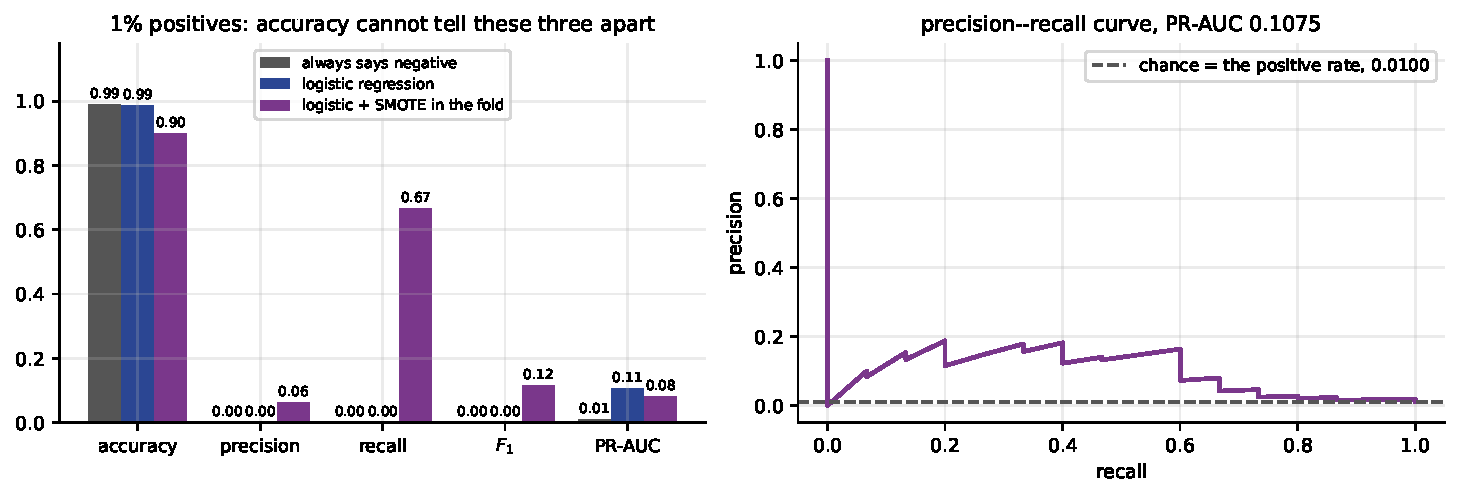
\includegraphics[width=0.86\textwidth]{imbalance.pdf}
  \caption{Left: five metrics for three models --- always-negative, plain
    logistic regression, and logistic regression with SMOTE. Accuracy is
    $0.99$, $0.99$, $0.90$: the one metric that barely distinguishes them is
    the one everybody quotes. Right: the precision--recall curve, whose
    baseline is the positive rate $0.01$.}
  \label{fig:imbalance}
\end{figure}

How bad does the imbalance have to be before this bites? There is no
threshold; it is a slope. Sweep the minority fraction from $50\%$ to $0.2\%$:

\begin{codeout}
imbalance ratio against what accuracy is worth
   minority  50.0% (2500 rows)  always-negative 0.5000  model accuracy 0.8586  recall 0.8704  PR-AUC 0.9063
   minority  20.0% (1000 rows)  always-negative 0.8000  model accuracy 0.8874  recall 0.6210  PR-AUC 0.7532
   minority  10.0% ( 500 rows)  always-negative 0.9000  model accuracy 0.9260  recall 0.4400  PR-AUC 0.6098
   minority   5.0% ( 250 rows)  always-negative 0.9500  model accuracy 0.9544  recall 0.2720  PR-AUC 0.4392
   minority   1.0% (  50 rows)  always-negative 0.9900  model accuracy 0.9890  recall 0.0400  PR-AUC 0.1916
   minority   0.2% (  10 rows)  always-negative 0.9980  model accuracy 0.9980  recall 0.0000  PR-AUC 0.0277
\end{codeout}

Two columns moving in opposite directions. As the problem gets harder,
\textbf{accuracy goes up} --- from $0.86$ at balance to $0.998$ at $0.2\%$ ---
while recall falls to zero. Reported accuracy on an imbalanced problem is
largely a measure of how imbalanced the problem is.

\subsection{Four things you can do about it}
\label{sec:four}

\begin{center}\small
\begin{tabular}{@{}lp{4.9cm}p{4.6cm}@{}}
  \toprule
  & \textbf{What it does} & \textbf{What it costs}\\
  \midrule
  \textbf{Random oversampling} & copies minority rows, with replacement, until
    the classes balance & exact duplicates: the model can memorise them\\[3pt]
  \textbf{Random undersampling} & throws majority rows away until the classes
    balance & discards most of your data\\[3pt]
  \textbf{SMOTE} & invents minority rows on the segments between existing ones
    & interpolates into regions where nothing was observed\\[3pt]
  \textbf{Class weights} & multiplies the loss of minority errors; no rows
    added or removed & nothing, and it is one keyword argument\\
  \bottomrule
\end{tabular}
\end{center}

And the one that is not on the list: \textbf{move the threshold}. A classifier
gives you a probability; $0.5$ is a convention, not a result. Choosing the
operating point from the precision--recall curve costs nothing and is often
all that is needed.

Written out, with no dependency on \texttt{imbalanced-learn}:

\begin{lstlisting}
rng = np.random.default_rng(0)      # the one seed for this lecture; every
                                    # resampler below is handed this rng


def random_oversample(X, y, rng):
    out_X, out_y = [X], [y]
    n_max = np.bincount(y).max()
    for c in np.unique(y):
        idx = np.where(y == c)[0]
        need = n_max - len(idx)
        if need > 0:
            pick = rng.choice(idx, size=need, replace=True)
            out_X.append(X[pick]); out_y.append(y[pick])
    return np.vstack(out_X), np.concatenate(out_y)

def random_undersample(X, y, rng):
    n_min = np.bincount(y).min()
    keep = np.concatenate([rng.choice(np.where(y == c)[0], size=n_min,
                                      replace=False) for c in np.unique(y)])
    rng.shuffle(keep)
    return X[keep], y[keep]
\end{lstlisting}

\subsection{SMOTE is one line of arithmetic}
\label{sec:smote}

\begin{worked}[SMOTE between two patients]
Two minority patients, $A = (1, 1)$ and $B = (3, 5)$. SMOTE draws
$u \sim \mathcal{U}(0,1)$ and returns the point $A + u(B - A)$:
\[
  u = 0 \to (1,1) = A, \quad
  u = \tfrac14 \to (1.5,\, 2), \quad
  u = \tfrac12 \to (2,\, 3), \quad
  u = 1 \to (3,5) = B.
\]
Check the middle one by hand: $B - A = (2, 4)$, so
$A + \tfrac12(2,4) = (1,1) + (1,2) = (2,3)$. That is the whole idea. Every
synthetic point lies on a straight segment between a real minority point and
one of its $k$ nearest minority neighbours.
\end{worked}

\begin{codeout}
SMOTE by hand between A = (1, 1) and B = (3, 5)
   u = 0.00  ->  A + u(B - A) = [1.0, 1.0]
   u = 0.25  ->  A + u(B - A) = [1.5, 2.0]
   u = 0.50  ->  A + u(B - A) = [2.0, 3.0]
   u = 1.00  ->  A + u(B - A) = [3.0, 5.0]
\end{codeout}

The whole of Chawla et al.\ (2002), in fifteen lines:

\begin{lstlisting}
def smote(X, y, rng, k=5, minority=1):
    Xmin = X[y == minority]
    n_need = int((y != minority).sum() - len(Xmin))
    if n_need <= 0:
        return X, y
    nn = NearestNeighbors(n_neighbors=min(k + 1, len(Xmin))).fit(Xmin)
    _, ind = nn.kneighbors(Xmin)
    ind = ind[:, 1:]                              # drop the point itself
    base_i = rng.integers(0, len(Xmin), n_need)
    nbr_i = ind[base_i, rng.integers(0, ind.shape[1], n_need)]
    u = rng.random((n_need, 1))
    new = Xmin[base_i] + u * (Xmin[nbr_i] - Xmin[base_i])
    return np.vstack([X, new]), np.concatenate([y, np.full(n_need, minority)])
\end{lstlisting}

\begin{keyidea}
SMOTE is not generating data. It is \textbf{asserting} that the straight line
between two ill patients is full of ill patients. Sometimes that is a
reasonable assumption. Sometimes --- categorical features, multi-modal
classes, minority points sitting inside a majority region --- it is exactly
wrong.
\end{keyidea}

What the three resamplers do to the $1\%$ problem, on a $3500$-row training
set:

\begin{codeout}
   random oversample   train  3500 ->  6930 rows,  class counts [3465, 3465]
   random undersample  train  3500 ->    70 rows,  class counts [35, 35]
   SMOTE               train  3500 ->  6930 rows,  class counts [3465, 3465]
      3430 of the 3465 minority rows are synthetic (99.0%)
      distinct minority rows: SMOTE 3465, oversampling 35
\end{codeout}

Read the last line twice. Oversampling turned $35$ patients into $3465$ rows
that are copies of \textbf{$35$ distinct patients}. SMOTE turned them into
$3465$ distinct points, but every one of them lies on a segment between two of
the same $35$. \textbf{Neither method has added a single new observation.}
Undersampling, meanwhile, kept $70$ of $3500$ rows --- $99.0\%$ of the
negatives thrown away.

\begin{figure}[htbp]
  \centering
  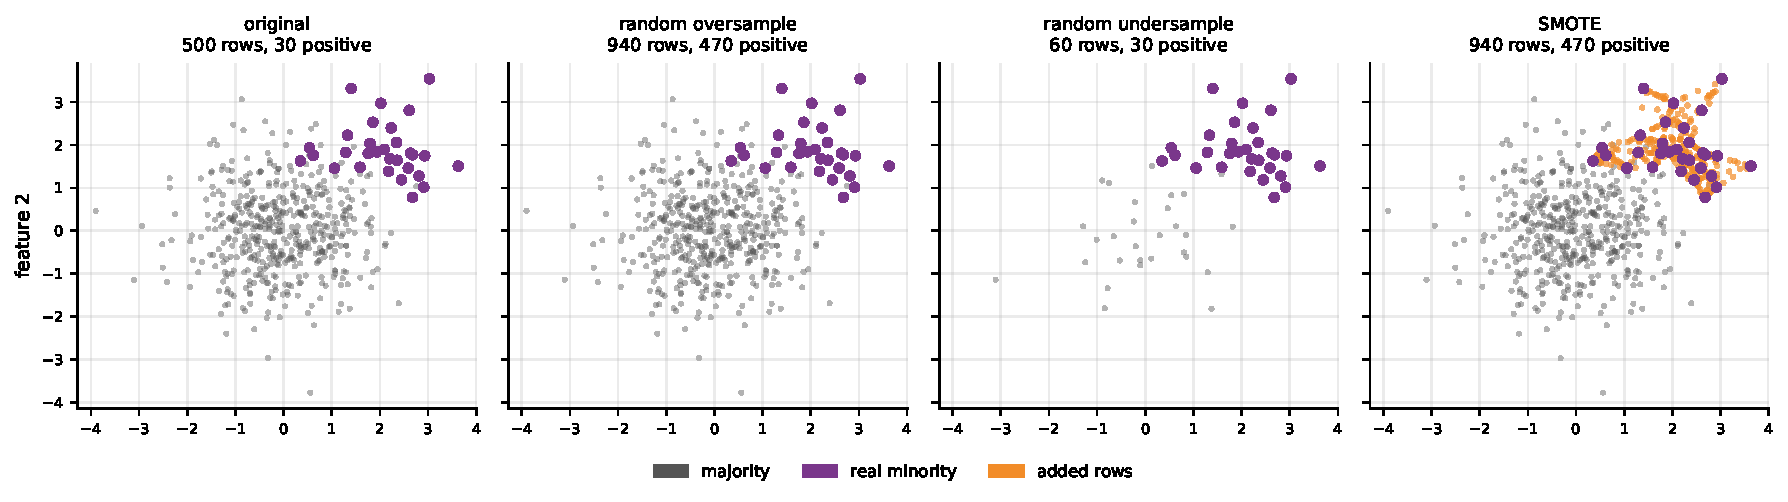
\includegraphics[width=0.92\textwidth]{resample.pdf}
  \caption{A two-dimensional version so you can see it. Purple is real
    minority, orange is added. Oversampling appears to add nothing --- the new
    points are exactly on top of the old ones. SMOTE's additions trace the
    segments between neighbours, which is why the cloud looks like a web.
    Undersampling simply deletes most of the majority class.}
  \label{fig:resample}
\end{figure}

\subsection{Does any of it help?}
\label{sec:doeshelp}

Five-fold stratified cross-validation, resampling applied \textbf{inside} each
fold to the training part only, logistic regression.

\begin{lstlisting}
def cv_imbalanced(X, y, make_model, resampler=None, k=5, seed=0):
    cv = StratifiedKFold(k, shuffle=True, random_state=seed)
    acc, pre, rec, f1s, ap = [], [], [], [], []
    for tr, te in cv.split(X, y):
        Xa, ya = X[tr], y[tr]
        if resampler is not None:                       # <-- INSIDE the fold,
            Xa, ya = resampler(Xa, ya, rng)             #     training part only
        m = make_model().fit(Xa, ya)
        p, s = m.predict(X[te]), m.predict_proba(X[te])[:, 1]
        acc.append(accuracy_score(y[te], p)); pre.append(precision_score(y[te], p))
        rec.append(recall_score(y[te], p));   f1s.append(f1_score(y[te], p))
        ap.append(average_precision_score(y[te], s))
    return [float(np.mean(v)) for v in (acc, pre, rec, f1s, ap)]
\end{lstlisting}
\begin{codeout}
   method                 accuracy precision  recall      F1   PR-AUC
   always negative         0.9900    0.0000  0.0000  0.0000   0.0100
   no treatment            0.9890    0.1333  0.0400  0.0583   0.1916
   random oversample       0.8542    0.0517  0.7800  0.0969   0.1369
   random undersample      0.7944    0.0390  0.8200  0.0744   0.1142
   SMOTE                   0.8814    0.0612  0.7600  0.1133   0.1404
   class_weight balanced   0.8556    0.0520  0.7800  0.0974   0.1368
\end{codeout}

Three things to take from this table, and the third one is the honest one.

\textbf{First}, recall moves enormously: $0.0400$ with no treatment, $0.76$ to
$0.82$ with any of the four. If your problem is ``find the ill patients'',
that is the difference between a useless model and a usable one.

\textbf{Second}, \texttt{class\_weight="balanced"} matches random oversampling
almost exactly --- recall $0.7800$ in both, accuracy $0.8556$ against
$0.8542$, $F_1$ $0.0974$ against $0.0969$. That is as it should be: weighting
a row by $w$ and including $w$ copies of it are the same thing to a loss
function that is a sum over rows. Prefer the class weight: no rows to manage,
no randomness, no opportunity to leak.

\textbf{Third, and this is the result to report rather than hide: none of the
four treatments improved PR-AUC.} The best PR-AUC in the table, $0.1916$,
belongs to the untreated model. Resampling moved the decision threshold; it
did not create information. The ranking of the test rows by predicted
probability --- which is what PR-AUC measures --- got slightly \emph{worse}.

\begin{caution}[Resampling is not free, and it is not a substitute for a threshold]
Everything the resamplers achieved on recall could have been achieved by
lowering the decision threshold on the untreated model, which is cheaper, has
no randomness in it, and leaves the probability estimates calibrated. Try that
first, and use the precision--recall curve to choose the operating point.
\end{caution}

The same table with a random forest instead is a useful corrective:

\begin{codeout}
does any of it help? the same table, random forest instead
   method                 accuracy precision  recall      F1   PR-AUC
   no treatment            0.9900    0.0000  0.0000  0.0000   0.2564
   random oversample       0.9900    0.1000  0.0200  0.0333   0.1981
   random undersample      0.7558    0.0359  0.9000  0.0691   0.1105
   SMOTE                   0.9876    0.2000  0.0800  0.1083   0.2056
   class_weight balanced   0.9900    0.0000  0.0000  0.0000   0.2769
\end{codeout}

The forest ranks better than the logistic regression did (PR-AUC $0.2564$
untreated, the best number anywhere in this lecture), and every resampler
except \texttt{class\_weight} made its ranking worse. Note also that
\texttt{class\_weight="balanced"} left the forest's \emph{predictions}
unchanged --- recall $0.0000$ with and without --- because for a tree ensemble
the weight enters the split criterion rather than a smooth additive loss, and
the majority vote at the leaves need not move at all. \textbf{Different model,
different answer. Measure; do not assume.}

\subsection{The mistake: resampling before the split}
\label{sec:resampleleak}

Everything above resampled inside the loop. Here is what happens when the same
line is written one level higher --- \texttt{X, y = smote(X, y)} before
\texttt{cross\_val\_score} instead of inside it. Nothing else changes: same
data, same model, same five folds.

\begin{lstlisting}
# WRONG
rng = np.random.default_rng(0)                    # the one seed
Xall, yall = smote(Xim, yim, rng)                 # the whole dataset
f1_bad = cross_val_score(mk(), Xall, yall, cv=cv, scoring="f1").mean()

# RIGHT: see cv_imbalanced above -- resample inside the loop
\end{lstlisting}
\begin{codeout}
the mistake: resample the WHOLE dataset, then cross-validate
   random oversample  BEFORE the split : F1 0.8607  recall 0.8655  PR-AUC 0.9176
   random oversample  INSIDE each fold : F1 0.0969  recall 0.7800  PR-AUC 0.1369
   random oversample  overstatement in F1 +0.7638
   SMOTE              BEFORE the split : F1 0.8942  recall 0.9067  PR-AUC 0.9207
   SMOTE              INSIDE each fold : F1 0.1133  recall 0.7600  PR-AUC 0.1404
   SMOTE              overstatement in F1 +0.7809
\end{codeout}

$F_1 = 0.8942$ against an honest $0.1133$. An eightfold overstatement, from
moving one line of code. And it is exactly the kind of number that makes a
report look finished, which is why it survives to submission.

Why does it happen? Look at what is in the test fold afterwards:

\begin{codeout}
   after oversampling before the split, fold 1 has 1980 test rows
   of which 990 (50.0%) are byte-identical to a training row
   among the 990 MINORITY test rows, 990 (100.0%) are copies
\end{codeout}

\textbf{Every single minority row in the test fold is a byte-identical copy of
a row the model trained on.} The model is not being tested; it is being asked
to remember. SMOTE is only slightly less blatant --- its synthetic points are
built \emph{from} the training points, using their coordinates and their
neighbourhood structure, so the same information crosses the boundary in a
less obvious form.

There is a second, quieter problem in that experiment even setting leakage
aside: after resampling the whole dataset the test folds are $50/50$ balanced.
That is not the balance you will meet in production, so even a leak-free score
computed on such a fold answers the wrong question.

\begin{figure}[htbp]
  \centering
  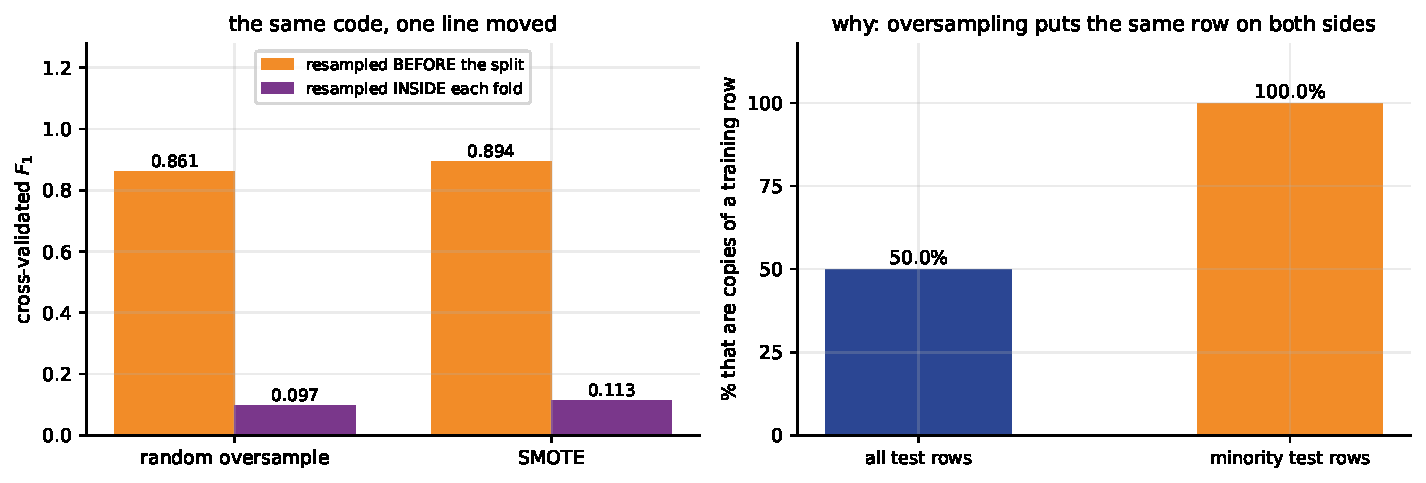
\includegraphics[width=0.86\textwidth]{resampleleak.pdf}
  \caption{Left: $F_1$ for both resamplers, before the split and inside the
    fold. Right: the mechanism --- half of every test fold, and \emph{all} of
    its minority half, are duplicates of training rows.}
  \label{fig:resampleleak}
\end{figure}

\begin{keyidea}[The rule, stated once]
\textbf{Resampling is part of the model.} It happens inside the fold, on the
training part only. The test fold keeps its natural class balance, because
that is the balance you will meet in production.
\end{keyidea}

This is the same rule as Lecture~6's rule about scalers and feature selection,
and it has the same one-line test: \emph{did this step look at the data?} If
yes, it belongs inside the loop. \texttt{imbalanced-learn}'s
\texttt{imblearn.pipeline.Pipeline} exists precisely because scikit-learn's own
\texttt{Pipeline} cannot hold a step that changes the number of rows; if you
resample by hand, you must place the call yourself, and this is where people
put it in the wrong place.

\subsection{The whole thing in one place}
\label{sec:whole}

Split, tune on the training part only, resample inside each inner fold, refit,
and report once on the test set.

\begin{lstlisting}
Xtr, Xte, ytr, yte = train_test_split(Xim, yim, test_size=0.3,
                                      stratify=yim, random_state=0)
cv = StratifiedKFold(5, shuffle=True, random_state=0)
best = (-1.0, None)
for C in [0.01, 0.1, 1, 10]:
    f1v = []
    for tr, va in cv.split(Xtr, ytr):
        Xa, ya = smote(Xtr[tr], ytr[tr], rng)          # inside the fold
        m = make_pipeline(StandardScaler(),
                          LogisticRegression(C=C, max_iter=5000)).fit(Xa, ya)
        f1v.append(f1_score(ytr[va], m.predict(Xtr[va])))   # va NOT resampled
    if np.mean(f1v) > best[0]:
        best = (float(np.mean(f1v)), C)
Xa, ya = smote(Xtr, ytr, rng)                     # refit on all training rows
final = make_pipeline(StandardScaler(),
                      LogisticRegression(C=best[1], max_iter=5000)).fit(Xa, ya)
\end{lstlisting}
\begin{codeout}
the whole thing in one place: split, tune, resample, evaluate
      C=  0.01  inner F1 0.1271
      C=  0.10  inner F1 0.1236
      C=  1.00  inner F1 0.1215
      C= 10.00  inner F1 0.1215
   chosen C=0.01 (inner F1 0.1271)
   held-out TEST: accuracy 0.8940  precision 0.0610  recall 0.6667  F1 0.1117  PR-AUC 0.0842
   confusion matrix [[1331, 154], [5, 10]]
\end{codeout}

Read the confusion matrix, not the decimals: \textbf{ten of the fifteen ill
patients found, at the cost of $154$ false alarms out of $1485$ healthy
people.} Whether that trade is acceptable is a clinical decision, not a
modelling one, and the most useful thing a modeller can do is state it in
those terms.

\begin{tryit}[Break it deliberately]
Take the block above and move the \texttt{smote} call to the line before
\texttt{train\_test\_split}. Everything else stays. You should see the held-out
$F_1$ leap from about $0.11$ to about $0.89$ --- and then convince yourself, by
checking for duplicate rows across the split, that the leap is entirely
fictitious. Doing this once, deliberately, is the best inoculation available.
\end{tryit}

% =========================================================================
\section{Summary}
\label{sec:summary}

\begin{enumerate}[leftmargin=*]
  \item A single train/test score is a \textbf{random variable}. On wine, $500$
    seeds gave $0.7556$ to $1.0000$; the middle $95\%$ spans $17$ points.
  \item That noise reverses model comparisons. Two trees differing by $0.0021$
    on average produced single-split verdicts from $+0.1556$ to $-0.1333$, and
    a ``winner'' on $193$ of $500$ splits.
  \item Test-set noise falls only as $1/\sqrt{n_{\text{te}}}$: sd $0.0425$ on
    $44$ test rows against $0.0214$ on $142$.
  \item \textbf{Stratify.} On a sorted $5\%$ file, \texttt{KFold} put all ten
    positives in fold~1, left fold~1's training set with one class, and
    reported mean accuracy $1.0000$ with mean recall $0.0000$.
  \item \textbf{Group.} Forty patients with coin-flip labels scored
    $1.0000 \pm 0.0000$ under a random split and $0.6483 \pm 0.1984$ under
    \texttt{GroupKFold}, because $37$ of $40$ patients appeared on both sides
    of fold~1.
  \item \textbf{Respect time.} A random split scored $R^2 = +0.9975$ where the
    honest time-ordered answer was $-2.8167$, and shuffled cross-validation
    ranked a useless model above a good one.
  \item $k$-fold costs $k$ fits. On $569$ rows, LOOCV costs $569$ fits
    against $5$-fold's $5$ --- $113.8\times$ as many, on any machine --- to
    reach the identical $0.9789$.
  \item Small $k$ is pessimistic because it starves the model: $2$-fold trains
    on $284$ rows, $20$-fold on $540$, and the learning curve between them is
    worth about $0.003$ here.
  \item \texttt{GridSearchCV.best\_score\_} is a \textbf{maximum}, not an
    estimate. On pure noise it read $0.5820$ against a nested $0.5265$; with a
    one-point grid the gap was exactly zero; with sixty points it was
    $+0.0783$.
  \item At $1\%$ positives, always-say-no scores $0.9900$ and a real model
    scores $0.9867$: \textbf{accuracy ranked the useless model higher}.
  \item Oversampling, undersampling, SMOTE and class weights all took recall
    from $0.0400$ to about $0.78$ --- and \textbf{none improved PR-AUC}. They
    move the threshold; they do not create information.
  \item \textbf{Resampling before the split reported $F_1 = 0.8942$ against an
    honest $0.1133$}, because $100\%$ of the minority test rows were copies of
    training rows.
\end{enumerate}

\begin{keyidea}[One sentence for the whole of Unit IV]
Anything you learn from the data --- a mean, a category list, a feature
subset, a hyper-parameter, a resampled row --- is part of the model, and
belongs inside the loop.
\end{keyidea}

% =========================================================================
\section{Practice questions}
\label{sec:questions}

\begin{enumerate}[leftmargin=*]
  \item \textbf{Folds by hand.} A dataset has $20$ rows, of which rows $17$,
    $18$ and $19$ (zero-indexed) are the only positives; the file is sorted.
    Write down the five test folds produced by \texttt{KFold(5)} and by
    \texttt{StratifiedKFold(5)}, and the number of positives in each. What
    goes wrong with the \texttt{KFold} version?

  \item \textbf{A confusion matrix.} A fraud detector on $10{,}000$
    transactions produces $\mathrm{TN} = 9900$, $\mathrm{FP} = 60$,
    $\mathrm{FN} = 30$, $\mathrm{TP} = 10$. Compute accuracy, precision,
    recall, $F_1$ and balanced accuracy. What accuracy would a model that
    always predicts ``not fraud'' achieve? Which single number would you put
    in the report, and why?

  \item \textbf{Cost.} For $n = 5000$ rows, compute the number of fits and the
    total number of row-fits for $2$-fold, $5$-fold, $10$-fold and LOOCV. If
    one fit on $4000$ rows takes $0.4$ seconds and cost scales linearly with
    rows, how long does each take?

  \item \textbf{Reporting.} Five hundred random $75/25$ splits of
    \texttt{load\_wine} gave a $2.5$th--$97.5$th percentile range of
    $[0.8106, 0.9778]$. A classmate reports ``our model achieves $97.8\%$
    accuracy''. Write the two-sentence reply you would give in a review, and
    state what you would ask them to run instead.

  \item \textbf{Choose the splitter.} For each of the following, name the
    splitter and give the reason in one line. (a) $12{,}000$ chest X-rays from
    $3000$ patients, predicting pneumonia. (b) Daily electricity demand for a
    campus, predicting tomorrow. (c) $600$ wine samples, three cultivars,
    roughly balanced. (d) $200{,}000$ card transactions, $0.17\%$ fraudulent,
    from $40{,}000$ cardholders, with a timestamp on every row. (e) $60$
    students' examination scripts marked by six examiners, with the examiner
    recorded.

  \item \textbf{SMOTE by hand.} Minority points $A = (2, 4)$ and
    $B = (6, 10)$, with $B$ the nearest minority neighbour of $A$. Compute the
    synthetic point for $u = 0.3$. Now suppose a third feature is
    ``blood group'', one-hot encoded as $(1,0,0)$ for $A$ and $(0,1,0)$ for
    $B$. What does SMOTE produce for that block at $u = 0.3$, and what is
    wrong with it?

  \item \textbf{Why \texttt{best\_score\_} is biased.} A grid has $m$
    combinations. Every one of them has the same true accuracy $\mu$, and the
    cross-validated estimate of each is $\mu + \varepsilon_i$ with the
    $\varepsilon_i$ independent and mean zero. Explain in three sentences why
    $\mathbb{E}[\max_i(\mu + \varepsilon_i)] > \mu$, and predict what happens
    to the bias as $m$ grows from $1$ to $60$. Check your prediction against
    the table in Section~\ref{sec:noise}.

  \item \textbf{Debug this.} A student reports: ``I have $2\%$ churners. I
    applied SMOTE to balance the dataset, then used \texttt{cross\_val\_score}
    with $5$-fold and got $F_1 = 0.89$. The model is ready to deploy.''
    Identify every error, say what the honest number is likely to look like,
    and write the corrected procedure as six numbered steps.

  \item \textbf{Debug this too.} A student predicting hourly air quality
    reports $R^2 = 0.998$ using \texttt{KFold(5, shuffle=True)} on three years
    of hourly readings, with features ``hour of day'', ``day of year'' and
    ``station id''. Explain the two independent problems with the evaluation,
    and describe the experiment that would show the score is an illusion.

  \item \textbf{Weights or copies?} \texttt{class\_weight="balanced"} and
    random oversampling gave nearly identical results for logistic regression
    in Section~\ref{sec:doeshelp}, but visibly different results for a random
    forest. Explain both observations. Which would you use in production, and
    what would you check before deciding?
\end{enumerate}

% =========================================================================
\section{Solutions}
\label{sec:solutions}

\paragraph{Solution 1.} By hand: \texttt{KFold(5)} on $20$ sorted rows takes
contiguous blocks of four, so the folds are $[0..3], [4..7], [8..11],
[12..15], [16..19]$ and \emph{all three} positives fall in fold~5.
\texttt{StratifiedKFold(5)} deals $17$ negatives and $3$ positives out
separately, so three folds get one positive each and two get none --- with
only three positives and five folds it cannot do better, and scikit-learn
warns that $n_{\text{splits}}$ exceeds the members of the smallest class.
Verified:

\begin{codeout}
20 rows, 3 positives.  StratifiedKFold(5) test folds:
   fold 1  test [0, 1, 2, 3]  positives 0
   fold 2  test [4, 5, 6, 7]  positives 0
   fold 3  test [8, 9, 10, 17]  positives 1
   fold 4  test [11, 12, 13, 18]  positives 1
   fold 5  test [14, 15, 16, 19]  positives 1
KFold(5, shuffle=False) on the same sorted array:
   fold 1  test [0, 1, 2, 3]  positives 0
   fold 2  test [4, 5, 6, 7]  positives 0
   fold 3  test [8, 9, 10, 11]  positives 0
   fold 4  test [12, 13, 14, 15]  positives 0
   fold 5  test [16, 17, 18, 19]  positives 3
\end{codeout}

What goes wrong: four of the five \texttt{KFold} folds contain no positive at
all, so recall is undefined on them and accuracy is trivially high; and the
fold that tests on rows $16$--$19$ trains on a set containing no positives, so
no classifier can be fitted. The deeper lesson is upstream of the splitter:
with three positives, \textbf{no} cross-validation scheme will give a usable
recall estimate. Collect more positives, or report the confusion matrix and
refuse to report a rate.

\paragraph{Solution 2.}
\begin{align*}
  \text{accuracy} &= \frac{10 + 9900}{10000} = 0.9910, &
  \text{precision} &= \frac{10}{10 + 60} = 0.1429,\\
  \text{recall} &= \frac{10}{10 + 30} = 0.2500, &
  F_1 &= \frac{2\,\mathrm{TP}}{2\,\mathrm{TP} + \mathrm{FP} + \mathrm{FN}}
      = \frac{20}{110} = 0.1818,
\end{align*}
and balanced accuracy $= \tfrac12(9900/9960 + 10/40) = \tfrac12(0.9940 +
0.2500) = 0.6220$. An always-negative model scores $9960/10000 = 0.9960$,
which is \emph{higher} than the real model's $0.9910$.

\begin{codeout}
   confusion matrix [[9900 60][30 10]]
   accuracy 0.9910  precision 0.1429  recall 0.2500  F1 0.1818
   an always-negative model would score accuracy 0.9960
   balanced accuracy 0.6220
\end{codeout}

Which number to report: none of them alone. Report the confusion matrix itself
--- ``we catch $10$ of $40$ frauds and raise $60$ false alarms'' --- and add
PR-AUC if a threshold-free summary is wanted. If forced to a single rate, use
recall or $F_1$; never accuracy.

\paragraph{Solution 3.} Row-fits are $k \cdot n(1 - 1/k) = n(k-1)$.

\begin{codeout}
cost of k-fold on n = 5000 rows
       2-fold:     2 fits, each on 2500 rows ->      5000 row-fits
       5-fold:     5 fits, each on 4000 rows ->     20000 row-fits
      10-fold:    10 fits, each on 4500 rows ->     45000 row-fits
     LOO-fold:  5000 fits, each on 4999 rows ->  24995000 row-fits
\end{codeout}

At $0.4$~s per fit on $4000$ rows the per-row cost is $10^{-4}$~s, so: $2$-fold
$0.5$~s, $5$-fold $2$~s, $10$-fold $4.5$~s, LOOCV $2499.5$~s --- about $42$
minutes. That is the honest reason nobody uses LOOCV on five thousand rows.

\paragraph{Solution 4.} Something like: ``$97.8\%$ is the upper end of the
range this experiment produces by chance --- five hundred re-runs of the same
code on the same data give anything from $81\%$ to $98\%$, so a single split
cannot distinguish your model from one that is seventeen points worse. Please
report a stratified $5$-fold or $10$-fold mean with its standard deviation,
and state the splitter and the seed.'' Verified spread:

\begin{codeout}
   500 seeds on wine: 95% of single splits land in [0.8106, 0.9778], width 0.1672
   a report of 1.0000 and a report of 0.7556 came from the same code
\end{codeout}

\paragraph{Solution 5.}
(a) \texttt{GroupKFold} or \texttt{StratifiedGroupKFold} grouped by
\emph{patient} --- four images of the same chest are near-duplicates.
(b) \texttt{TimeSeriesSplit} --- a model that trains on next month to predict
this month is not a forecaster.
(c) \texttt{StratifiedKFold(5, shuffle=True)} --- independent rows, and
stratifying costs nothing even when the classes are near-balanced.
(d) \texttt{TimeSeriesSplit} first, because fraud patterns drift and you must
predict forward; then check group leakage by cardholder, and use group-aware
splitting if a single cardholder carries many of the frauds. When constraints
conflict, the time constraint wins --- it is the one that mirrors deployment.
(e) \texttt{GroupKFold} grouped by \emph{examiner} if you are modelling marks,
because examiner severity is a shared effect; group by student instead if the
row unit is a question within a script.

\paragraph{Solution 6.} $B - A = (4, 6)$, so the synthetic point is
$A + 0.3(4,6) = (2, 4) + (1.2, 1.8) = (3.2,\, 5.8)$.

For the one-hot block, SMOTE interpolates each coordinate independently:
$(1,0,0) + 0.3\big((0,1,0) - (1,0,0)\big) = (0.7,\, 0.3,\, 0)$. That is a
patient who is $70\%$ blood group A and $30\%$ blood group B --- a row that
cannot exist. Interpolation is only meaningful for continuous features. The
remedies are SMOTE-NC (which takes the majority category among the neighbours
rather than averaging), or resampling only on the numeric block, or ---
usually best --- using class weights instead.

\paragraph{Solution 7.} The maximum of $m$ random variables is at least as
large as any one of them, and strictly larger whenever they differ, so
$\mathbb{E}[\max_i(\mu + \varepsilon_i)] \ge \mu + \mathbb{E}[\varepsilon_1]
= \mu$, with strict inequality as soon as the $\varepsilon_i$ have any spread.
The selected value carries the noise that made it the winner, so re-measuring
it on fresh folds regresses it back towards $\mu$. For roughly Gaussian noise
of sd $\sigma$ the expected maximum grows like $\mu + \sigma\sqrt{2\ln m}$:
slowly, but without bound, so bigger grids buy bigger illusions. The measured
table agrees: $+0.0000$ at $m = 1$, $+0.0200$ at $4$, $+0.0617$ at $20$,
$+0.0783$ at $60$.

\paragraph{Solution 8.} Errors: (i) SMOTE was applied to the whole dataset
before splitting, so synthetic test rows were built from training rows --- the
leak of Section~\ref{sec:resampleleak}, worth $+0.7809$ of $F_1$ in the
measured case; (ii) the test folds are $50/50$ after resampling, so even a
leak-free score would answer the wrong question; (iii) no held-out test set
exists at all, only cross-validation used both for choosing and for reporting;
(iv) $F_1$ alone hides the precision/recall trade-off that a churn team must
actually choose. The honest number for a $2\%$ minority is far more likely to
lie in the $0.1$--$0.3$ range than at $0.89$.

Corrected procedure: (1) split off a stratified test set and put it away;
(2) build a stratified $k$-fold loop on the training part; (3) inside each
fold, fit the scaler and resample \emph{the training part of that fold only};
(4) score on the untouched validation part, using recall, precision, $F_1$ and
PR-AUC; (5) choose hyper-parameters --- including whether to resample at all
--- by the inner loop, and pick the operating threshold from the
precision--recall curve; (6) refit on all the training rows with the chosen
settings and report on the test set, once, with the confusion matrix.

\paragraph{Solution 9.} Two independent problems. \textbf{Time}: with
\texttt{shuffle=True} on three years of hourly data, almost every test hour
sits between two training hours, so the model interpolates rather than
forecasts, while the deployment task is extrapolation. \textbf{Groups and
features}: ``hour of day'' plus ``day of year'' plus ``station id'' identifies
a specific hour at a specific station almost uniquely across three years, so
the model can memorise a lookup table. Together these give a score that says
nothing about tomorrow.

The experiment that shows it: refit with \texttt{TimeSeriesSplit(5)} and
compare. Section~\ref{sec:time} is exactly this experiment on synthetic data,
and it moved $R^2$ from $+0.9975$ to $-2.8167$. Then, as a second check, hold
out the last three months entirely and predict them; a model that scores well
on shuffled folds and badly here is memorising.

\paragraph{Solution 10.} For logistic regression the loss is a sum of per-row
terms, so multiplying a row's term by $w$ and including $w$ copies of that row
are algebraically the same thing, up to the randomness in which rows get
copied. Hence the near-identical numbers: recall $0.7800$ for both, accuracy
$0.8556$ against $0.8542$.

For a random forest the weight enters the impurity computation at each split
and the bootstrap sampling, not a smooth additive loss; and the final
prediction is a majority vote at the leaves, which a weight need not change at
all. That is why \texttt{class\_weight="balanced"} left the forest's
predictions identical to the untreated forest (recall $0.0000$ in both) while
oversampling and undersampling moved them.

In production: prefer \texttt{class\_weight}. It adds no rows, adds no
randomness, cannot leak across a split, costs nothing in memory or time, and
is a single keyword argument. Before deciding, check three things --- that the
model supports it (\texttt{class\_weight} or \texttt{sample\_weight}), that
PR-AUC does not get worse (in Section~\ref{sec:doeshelp} it did), and whether
simply moving the threshold on the untreated model achieves the same recall
more cheaply. It usually does.

% =========================================================================
\section{References and further reading}
\label{sec:refs}

All links were checked on 22 August 2026. Free resources are marked
\textbf{[free]}.

\subsection*{Textbooks}

\begin{itemize}[leftmargin=*]
  \item M\"uller and Guido, \emph{Introduction to Machine Learning with
    Python}, O'Reilly, 2016. \textbf{The prescribed text for this lecture.}
    \S5.1 cross-validation --- \S5.1.1 cross-validation in scikit-learn,
    \S5.1.2 the benefits of cross-validation, \S5.1.3 stratified $k$-fold and
    the other splitters (leave-one-out, shuffle-split,
    \texttt{GroupKFold}); then \S5.2 grid search, \S5.2.4 nested
    cross-validation, and \S5.3.2 on metrics for imbalanced binary
    classification. Notebooks \textbf{[free]}:
    \url{https://github.com/amueller/introduction_to_ml_with_python}
  \item James, Witten, Hastie, Tibshirani and Taylor, \emph{An Introduction to
    Statistical Learning with Python}. \textbf{[free]} Ch.~5, ``Resampling
    Methods'': \S5.1.1 the validation-set approach and its variability --- the
    same experiment as Section~\ref{sec:spread}; \S5.1.2 LOOCV; \S5.1.3
    $k$-fold; \S5.1.4 the bias--variance trade-off for $k$; \S5.1.5
    cross-validation for classification; \S5.2 the bootstrap. The lab at the
    end of the chapter is worth doing in full.
    \url{https://www.statlearning.com/}
  \item Han, Kamber and Pei, \emph{Data Mining: Concepts and Techniques}, 3rd
    edition, Morgan Kaufmann, 2012. \S8.5 on evaluating classifier accuracy
    --- \S8.5.1 the confusion matrix and the derived measures, \S8.5.2 holdout
    and random subsampling, \S8.5.3 cross-validation, \S8.5.4 the bootstrap;
    \textbf{\S8.6} on comparing classifiers, significance tests and ROC
    curves; and \S8.6.5 on the class-imbalance problem, which is where the
    oversampling/undersampling vocabulary of the syllabus comes from.
  \item Hastie, Tibshirani and Friedman, \emph{The Elements of Statistical
    Learning}, 2e, Springer. Ch.~7 is the definitive treatment: \S7.10
    cross-validation, and above all \textbf{\S7.10.2, ``The Wrong and Right
    Way to Do Cross-validation''}, which is Section~\ref{sec:nested} of these
    notes written twenty years earlier.
  \item Kuhn and Johnson, \emph{Applied Predictive Modeling}, Springer. Ch.~4
    on over-fitting and resampling --- a very clear account of why repeated
    $k$-fold beats a single split --- and Ch.~16 on remedies for class
    imbalance, including sampling methods and cost-sensitive training.
  \item Kuhn and Johnson, \emph{Feature Engineering and Selection}.
    \textbf{[free]} \S3.4 on resampling, and Ch.~10--11 on the selection bias
    that Lecture~6 measured and this lecture explains.
    \url{http://www.feat.engineering/}
\end{itemize}

\subsection*{Online courses}

\begin{sloppypar}
\begin{itemize}[leftmargin=*]
  \item \textbf{NPTEL, Introduction to Machine Learning} --- Prof.\ Balaraman
    Ravindran, IIT Madras. The reference course for this semester; the
    evaluation-measures and cross-validation lectures use the vocabulary the
    examination uses. \textbf{[free]}
    \url{https://nptel.ac.in/courses/106106139}
  \item \textbf{NPTEL, Data Mining} --- Prof.\ Pabitra Mitra, IIT Kharagpur.
    The classifier-evaluation lectures match Han, Kamber and Pei
    \S8.5--8.6 section for section. \textbf{[free]}
    \url{https://nptel.ac.in/courses/106105174}
  \item \textbf{SWAYAM} --- the national portal that hosts NPTEL, with
    certification. \textbf{[free]} \url{https://swayam.gov.in/}
  \item \textbf{Kaggle Learn, Intermediate Machine Learning} --- seven short
    browser lessons; the \emph{Cross-Validation} lesson and the \emph{Data
    Leakage} lesson together are the practical companion to this entire
    lecture, and take about an hour. \textbf{[free]}
    \url{https://www.kaggle.com/learn/intermediate-machine-learning}
  \item \textbf{Google Machine Learning Crash Course} --- the
    \emph{Classification} module (thresholds and the confusion matrix;
    accuracy, recall, precision; ROC and AUC) and the \emph{Datasets,
    generalization, and overfitting} module (imbalanced datasets; dividing the
    original dataset). \textbf{[free]}
    \url{https://developers.google.com/machine-learning/crash-course/classification}
    \\
    \url{https://developers.google.com/machine-learning/crash-course/overfitting/imbalanced-datasets}
\end{itemize}
\end{sloppypar}

\subsection*{Videos}

\begin{itemize}[leftmargin=*]
  \item StatQuest with Josh Starmer, \emph{Machine Learning Fundamentals:
    Cross Validation} --- six minutes, and the clearest available picture of
    why you rotate the test fold. Watch before Section~\ref{sec:cv}.
    \textbf{[free]} \url{https://youtu.be/fSytzGwwBVw}
  \item StatQuest with Josh Starmer, \emph{Machine Learning Fundamentals: The
    Confusion Matrix} --- the table of Section~\ref{sec:imbal} built up one
    cell at a time. \textbf{[free]} \url{https://youtu.be/Kdsp6soqA7o}
  \item StatQuest with Josh Starmer, \emph{ROC and AUC, Clearly Explained!}
    --- what moving the threshold does, which is the operation every resampler
    in Section~\ref{sec:four} is imitating. \textbf{[free]}
    \url{https://youtu.be/4jRBRDbJemM}
  \item Mahesh Huddar, \emph{K-Fold Cross Validation, Stratified K-Fold,
    Leave-one-out Leave-P-Out Cross Validation} --- the splitters worked
    through in examination vocabulary, with a numerical example.
    \textbf{[free]} \url{https://youtu.be/PF2wLKv2lsI}
  \item CampusX, \emph{Imbalanced Data in Machine Learning $\vert$
    Undersampling $\vert$ Oversampling $\vert$ SMOTE} --- the remedies of
    Section~\ref{sec:four} demonstrated in Python. \textbf{[free]}
    \url{https://youtu.be/yh2AKoJCV3k}
\end{itemize}

\subsection*{Documentation and interactive explainers}

\begin{itemize}[leftmargin=*]
  \item scikit-learn user guide, \emph{Cross-validation: evaluating estimator
    performance} (\S3.1) --- the authoritative list of splitters, with the
    ``visualizing cross-validation behavior'' example that
    Figure~\ref{fig:cvsplits} is modelled on; and \emph{Tuning the
    hyper-parameters of an estimator} (\S3.2), whose nested-CV example is
    Section~\ref{sec:nested}. \textbf{[free]}
    \url{https://scikit-learn.org/stable/modules/cross_validation.html} \\
    \url{https://scikit-learn.org/stable/modules/grid_search.html} \\
    \url{https://scikit-learn.org/stable/auto_examples/model_selection/plot_cv_indices.html}
    \\
    \url{https://scikit-learn.org/stable/auto_examples/model_selection/plot_nested_cross_validation_iris.html}
  \item scikit-learn, \emph{Common pitfalls and recommended practices} --- read
    the data-leakage section before you next report a score. \textbf{[free]}
    \url{https://scikit-learn.org/stable/common_pitfalls.html}
  \item scikit-learn user guide, \emph{Metrics and scoring} (\S3.4) --- the
    definitions of precision, recall, $F_\beta$, balanced accuracy, average
    precision and the ROC and PR curves used throughout
    Section~\ref{sec:imbal}. \textbf{[free]}
    \url{https://scikit-learn.org/stable/modules/model_evaluation.html}
  \item \emph{imbalanced-learn} documentation --- the over-sampling,
    under-sampling and metrics chapters, and in particular \S9, \emph{Common
    pitfalls and recommended practices}, which demonstrates the leak of
    Section~\ref{sec:resampleleak} on a real dataset and shows the
    \texttt{imblearn.pipeline.Pipeline} that prevents it. \textbf{[free]}
    \url{https://imbalanced-learn.org/stable/common_pitfalls.html} \\
    \url{https://imbalanced-learn.org/stable/over_sampling.html}
  \item MLU-Explain, \emph{Train, Test, and Validation Sets} --- an
    interactive explainer; drag the points and watch the three sets do
    different jobs. The best five minutes you can spend on
    Section~\ref{sec:nested}. \textbf{[free]}
    \url{https://mlu-explain.github.io/train-test-validation/}
\end{itemize}

\subsection*{Articles}

\begin{itemize}[leftmargin=*]
  \item Chawla, Bowyer, Hall and Kegelmeyer, ``SMOTE: Synthetic Minority
    Over-sampling Technique'', \emph{Journal of Artificial Intelligence
    Research} \textbf{16} (2002), 321--357. \textbf{[free]} The paper
    Section~\ref{sec:smote} implements; the algorithm itself occupies half a
    page. \url{https://www.jair.org/index.php/jair/article/view/10302}
  \item Cawley and Talbot, ``On Over-fitting in Model Selection and Subsequent
    Selection Bias in Performance Evaluation'', \emph{Journal of Machine
    Learning Research} \textbf{11} (2010), 2079--2107. \textbf{[free]} The
    definitive study of the optimism measured in Section~\ref{sec:noise}, with
    the argument for nested cross-validation.
    \url{https://www.jmlr.org/papers/v11/cawley10a.html}
\end{itemize}

\enlargethispage{4\baselineskip}
\notesources{\AMLUnitIVSources}

\end{document}
